\documentclass{beamer}
\usepackage{amsthm}
\usepackage{amsmath}
\usepackage{amsfonts}
\usepackage{amssymb}
\usepackage{epic}
\usepackage{graphicx}
\usepackage{epstopdf}
\usepackage{multirow}
\usetheme{Berlin}
\usecolortheme{seahorse}
\usepackage{multicol}



\newtheorem{question}{Question}[section] 

\title{Project 3: \emph{"Brought to you by the letter ..."} }



\author{Andrew Bernath, Heather Kitada, Ethan Edwards}



\institute{Oregon State University}



\begin{document}

\begin{frame}
\titlepage
\end{frame}



\begin{frame}{\contentsname}
\begin{multicols}{2}
\tableofcontents
\end{multicols}
\end{frame}

\section{Introduction and Overview}
\begin{frame}
\frametitle{Question of Interest}
\large{\emph{Classify an image of a letter to one of the 26 capital letters in the English alphabet.}}

\begin{center} 
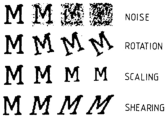
\includegraphics[width=.6 \textwidth]{letterDistortion}

\tiny{http://imagebank.osa.org/getImage.xqy?img=dTcqLmxhcmdlLGFvLTIzLTEwLTE1MDktZzAxMA}
\end{center}
\end{frame}

\subsection{Data Set Information}
\begin{frame}
\frametitle{Data Set Information}
\begin{itemize}
\item All 26 uppercase English letters 
\item 20 fonts for each letter 
\item Randomly distorted 
\begin{itemize}
\item File of 20,000 unique observations
\end{itemize}
\item Each observation converted into 16 primitive numerical attributes 
\end{itemize}
\end{frame}

\subsection{Variables}
\begin{frame}
16 Variables Used:

\begin{enumerate}
\item \small{\textbf{lettr}: True capital letter	(26 values from A to Z) }
\item \small{\textbf{x-box}:  Horizontal position of box	(integer) }
\item \small{\textbf{y-box}:	Vertical position of box	(integer) }
\item \small{\textbf{width}:	Width of box	 (integer) }
\item \small{\textbf{high}: Height of box	 (integer) }
\item \small{\textbf{onpix}:	Total number on pixels	 (integer) }
\item \small{\textbf{x-bar}:	Mean $x$ of on pixels in box	(integer) }
\item \small{\textbf{y-bar}:	Mean $y$ of on pixels in box	(integer) }
\item \small{\textbf{x2bar}:	Mean $x$ variance	 (integer) }
\item \small{\textbf{y2bar}:	Mean $y$ variance	 (integer) }
\item \small{\textbf{xybar}:	Mean $xy$ correlation	 (integer) }
\item \small{\textbf{x2ybr}:	Mean of $xxy$	 (integer) }
\item \small{\textbf{xy2br}:	Mean of $xyy$	 (integer) }
\item \small{\textbf{x-ege}:	Mean edge count left to right	(integer) }
\item \small{\textbf{xegvy}:	Correlation of $x$-ege with $y$	(integer) }
\item \small{\textbf{y-ege}:	Mean edge count bottom to top	(integer) }
\item \small{\textbf{yegvx}:	Correlation of $y$-ege with $x$	(integer)}
\end{enumerate}
\end{frame}

\section{Description of Methods}
\begin{frame}
\frametitle{Description of Methods}

Algorithms for:
\begin{enumerate}
\item Logistic Regression Binary Search Tree (BST)
\item Decision Trees for Classification
\begin{enumerate}
\item CART Method
\item Bag Method 
\end{enumerate}
\end{enumerate}
\end{frame}

\subsection{Logistic Regression BST Algorithm}
\begin{frame}
\frametitle{Logistic Regression BST Algorithm}
Preparing Binary Tree (Using Learning Set):
\begin{enumerate}
\item \small{Summarize by unique letter (average over observations from a given letter for each of the metrics)}
\item \small{Find distance between letters (uses Euclidean distance)}
\item \small{Use hclust() with "complete" method to create dendrogram}
\end{enumerate}
\begin{center} 
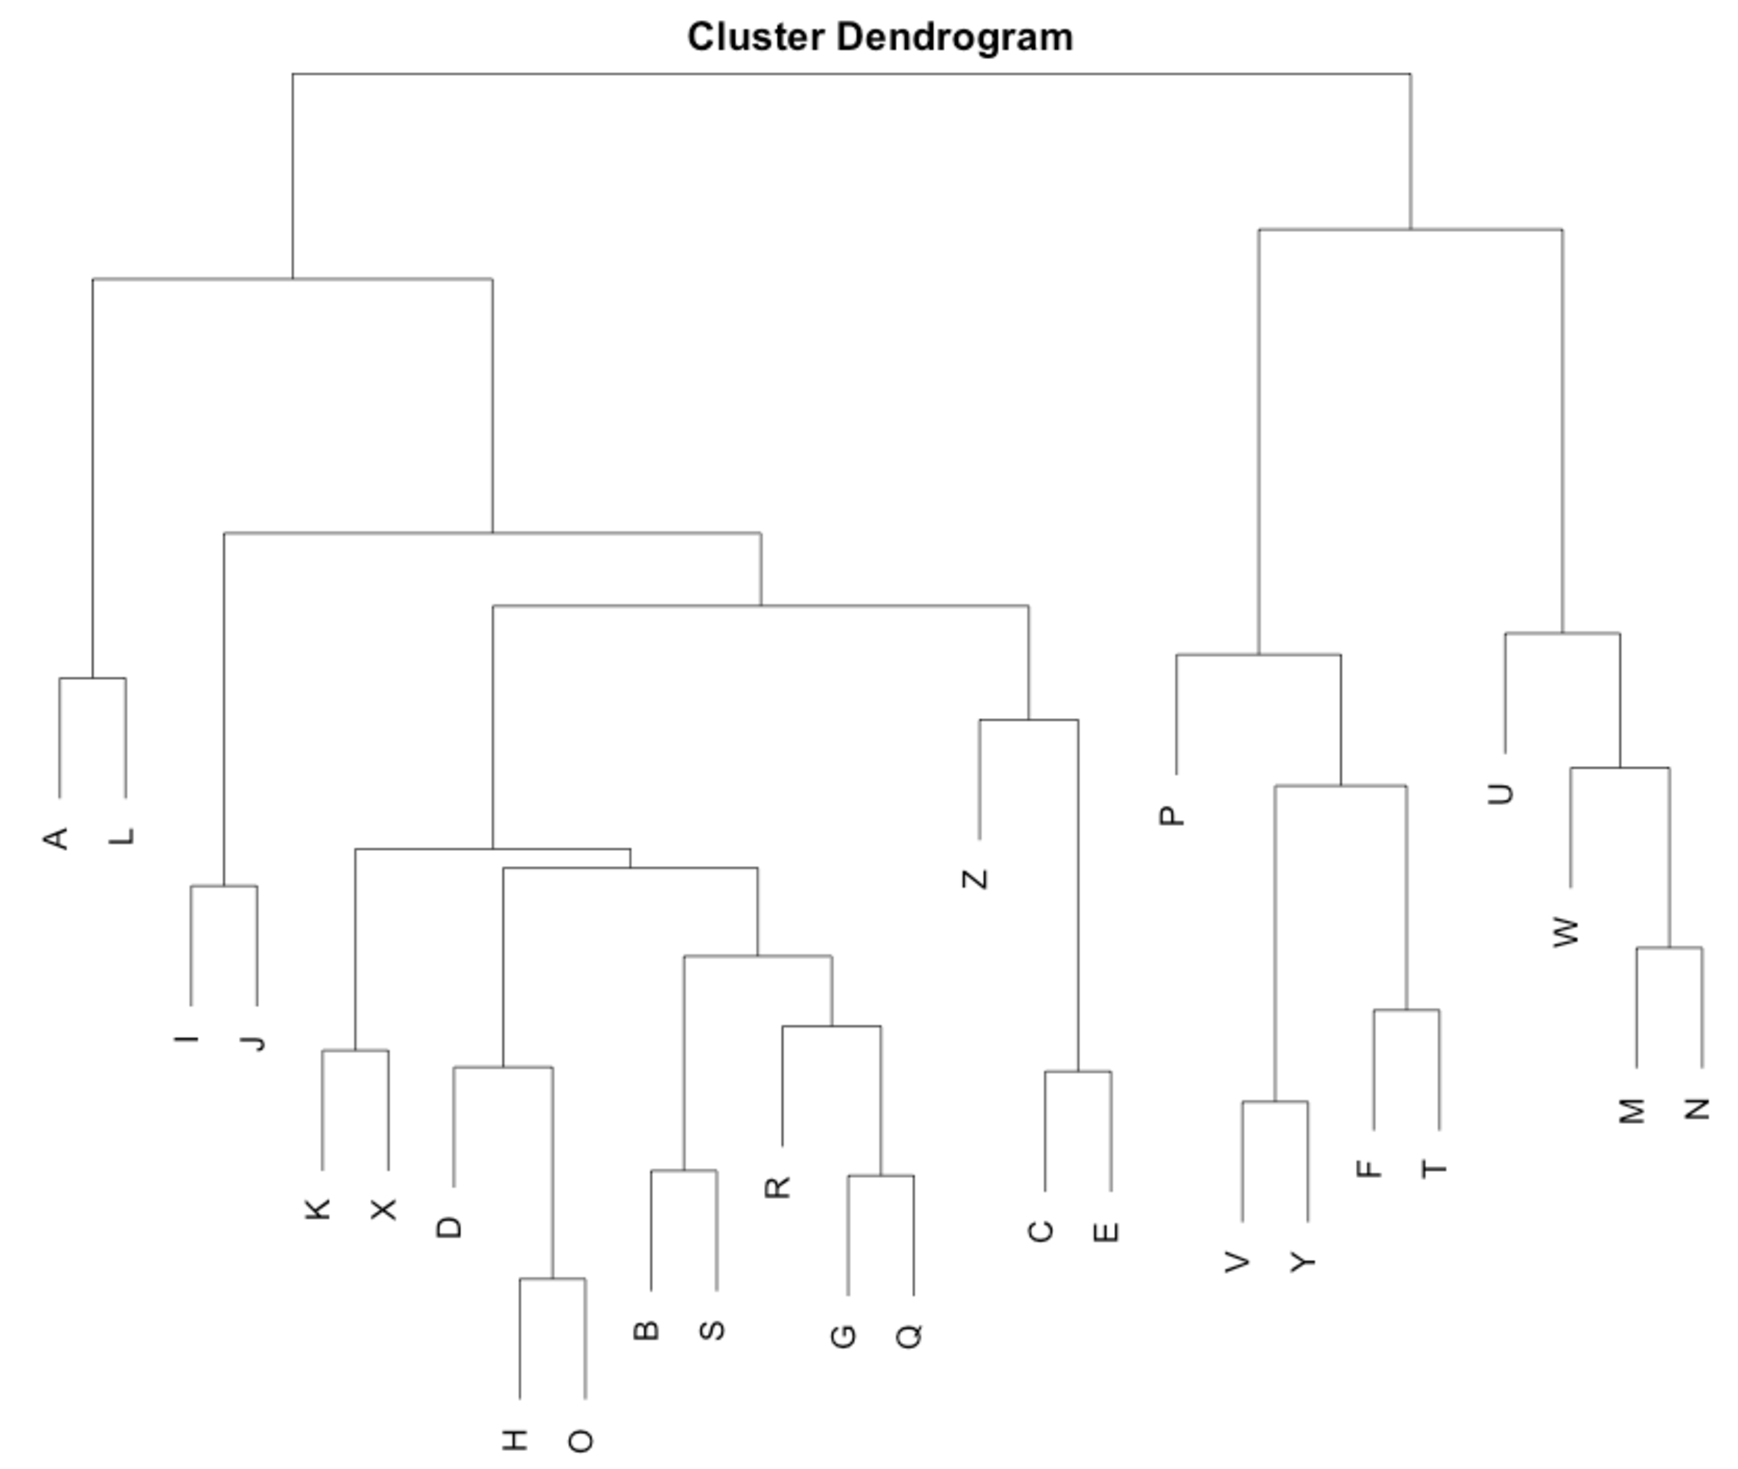
\includegraphics[width=.45 \textwidth]{letterDendrogram}
\end{center}
\end{frame}

\begin{frame}
\frametitle{Logistic Regression BST Algorithm}
Traversing Binary Tree with Logistic Regression Models:
\begin{enumerate}
\item \small{Subset letters are to the left and right of current intersection location.} \small{Right letters = 1, Left letters = 0}
\item \small{Create logistic regression model for probability of right (uses all 15 explanatory variables)}
\item \small{Evaluate logistic regression model with new covariates from observation in validation set. }
 \begin{displaymath}
\left\{
     \begin{array}{lr}
       \text{move right} & : \text{if } \hat{\pi} \geq 0.5\\
      \text{move left} & : \text{if } \hat{\pi} < 0.5
     \end{array}
   \right.
\end{displaymath} 
\item \small{Keep track of path traversed}
\item \small{Repeat steps 1-4 until you arrived at an end node, which is the predicted letter}
\end{enumerate}

\end{frame}

\begin{frame}
\frametitle{\small{Logistic Regression BST Algorithm Example}}
\small{New observation: ( T, 2,     6,     3,    4,     2,     7,    12,      2,      7,      7,      11,       8,     1,11,     1,      8)}
\begin{center} 
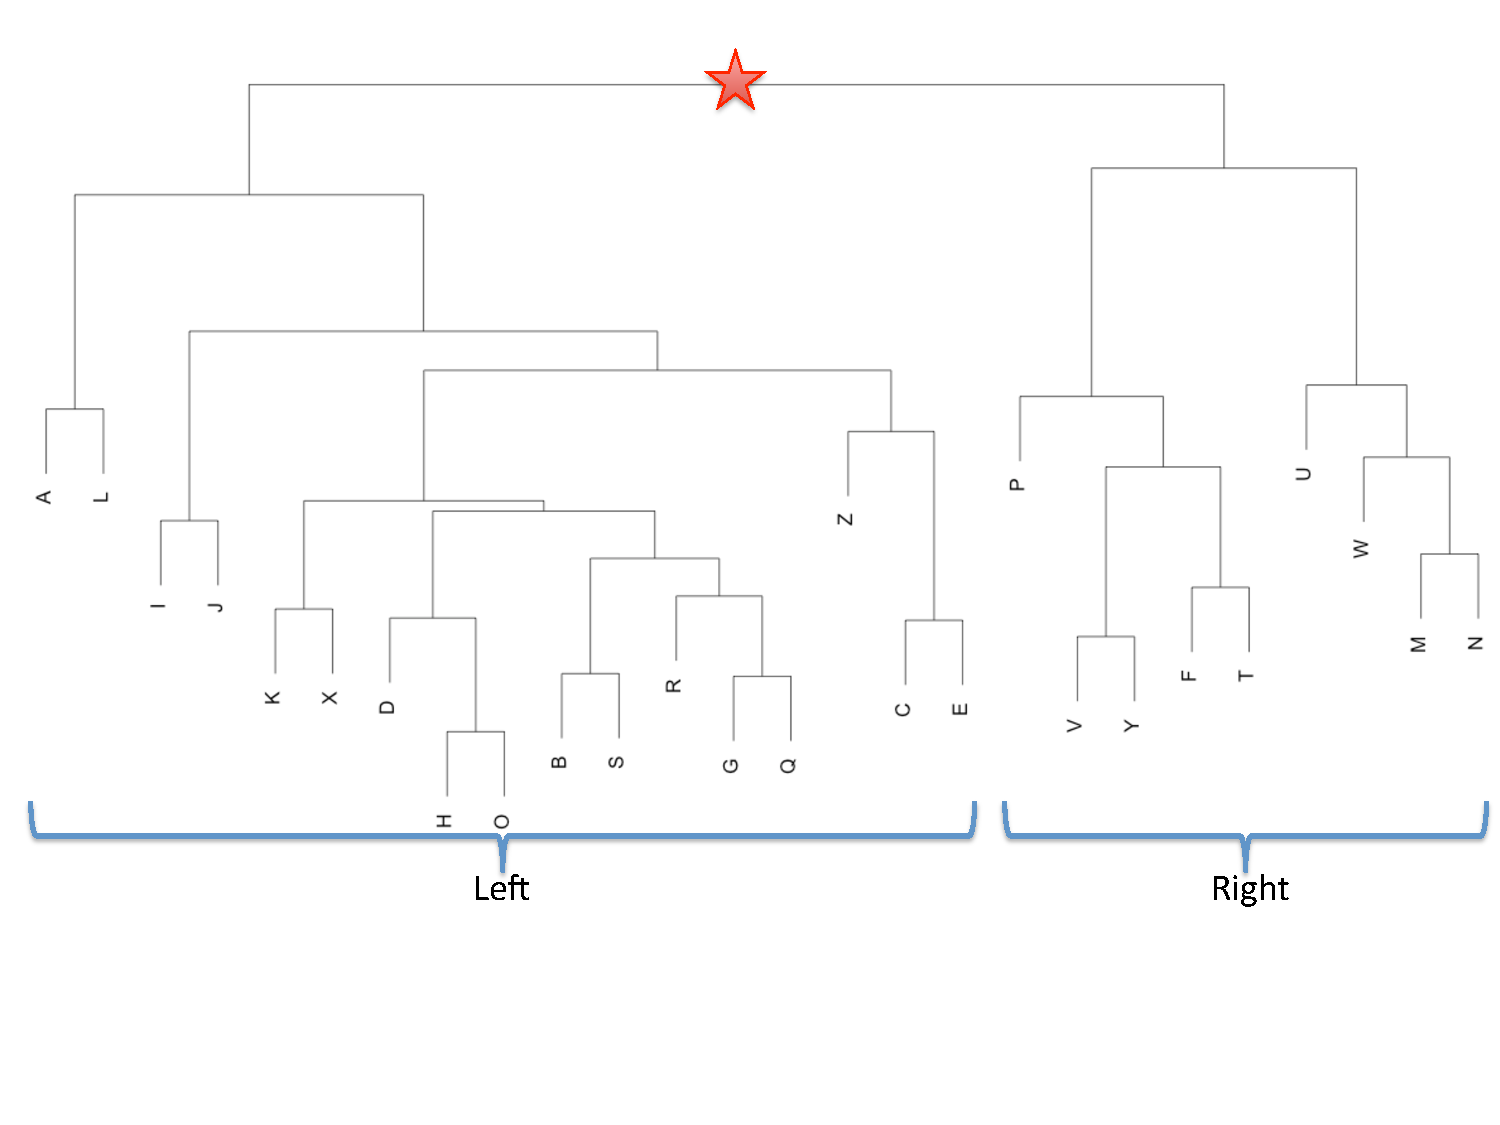
\includegraphics[width=.7 \textwidth]{firstStep}

\tiny{$log(\frac{\pi_i}{1-\pi_i})= -.5+.32x_1-.08x_2+.07x_3-.1x_4+.11x_5-.05x_6+.41x_7-.09x_8-.3x_{9}-.05x_{10}+.54x_{11}-.68x_{12}+.56x_{13}+.23x_{14}-.58x_{15}-.24x_{16} \rightarrow \hat{\pi}=0.929$}
\end{center}
Move right!

\end{frame}

\begin{frame}
\frametitle{\small{Logistic Regression BST Algorithm Example}}
\small{New observation: ( T, 2,     6,     3,    4,     2,     7,    12,      2,      7,      7,      11,       8,     1,11,     1,      8)}
\begin{center} 
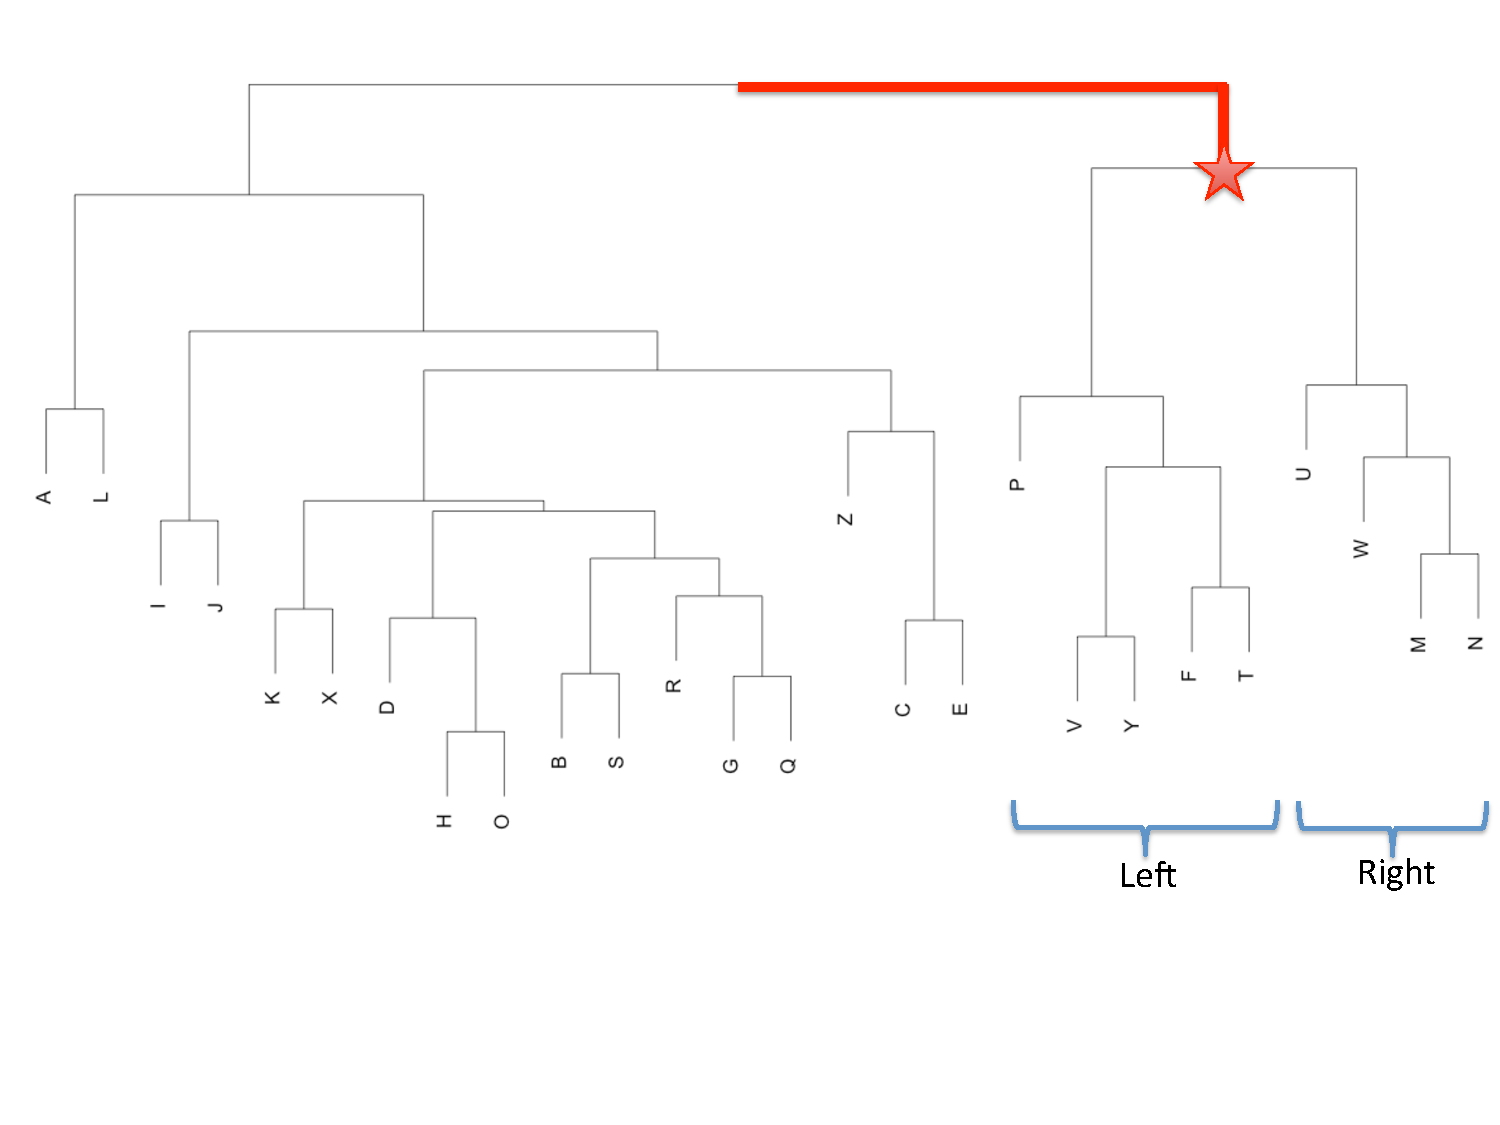
\includegraphics[width=.7 \textwidth]{secondStep}

\tiny{$log(\frac{\pi_i}{1-\pi_i})= 4.12-.37x_1+.15x_2+.83x_3-1.07x_4+.3x_5-.64x_6+.23x_7+1.17x_8+.58x_{9}-.39x_{10}-.83x_{11}+.88x_{12}+1.87x_{13}-.51x_{14}-2x_{15}-.57x_{16} \rightarrow \hat{\pi}=0.0007$}
\end{center}
Move left!

\end{frame}

\begin{frame}
\frametitle{\small{Logistic Regression BST Algorithm Example}}
\small{New observation: ( T, 2,     6,     3,    4,     2,     7,    12,      2,      7,      7,      11,       8,     1,11,     1,      8)}
\begin{center} 
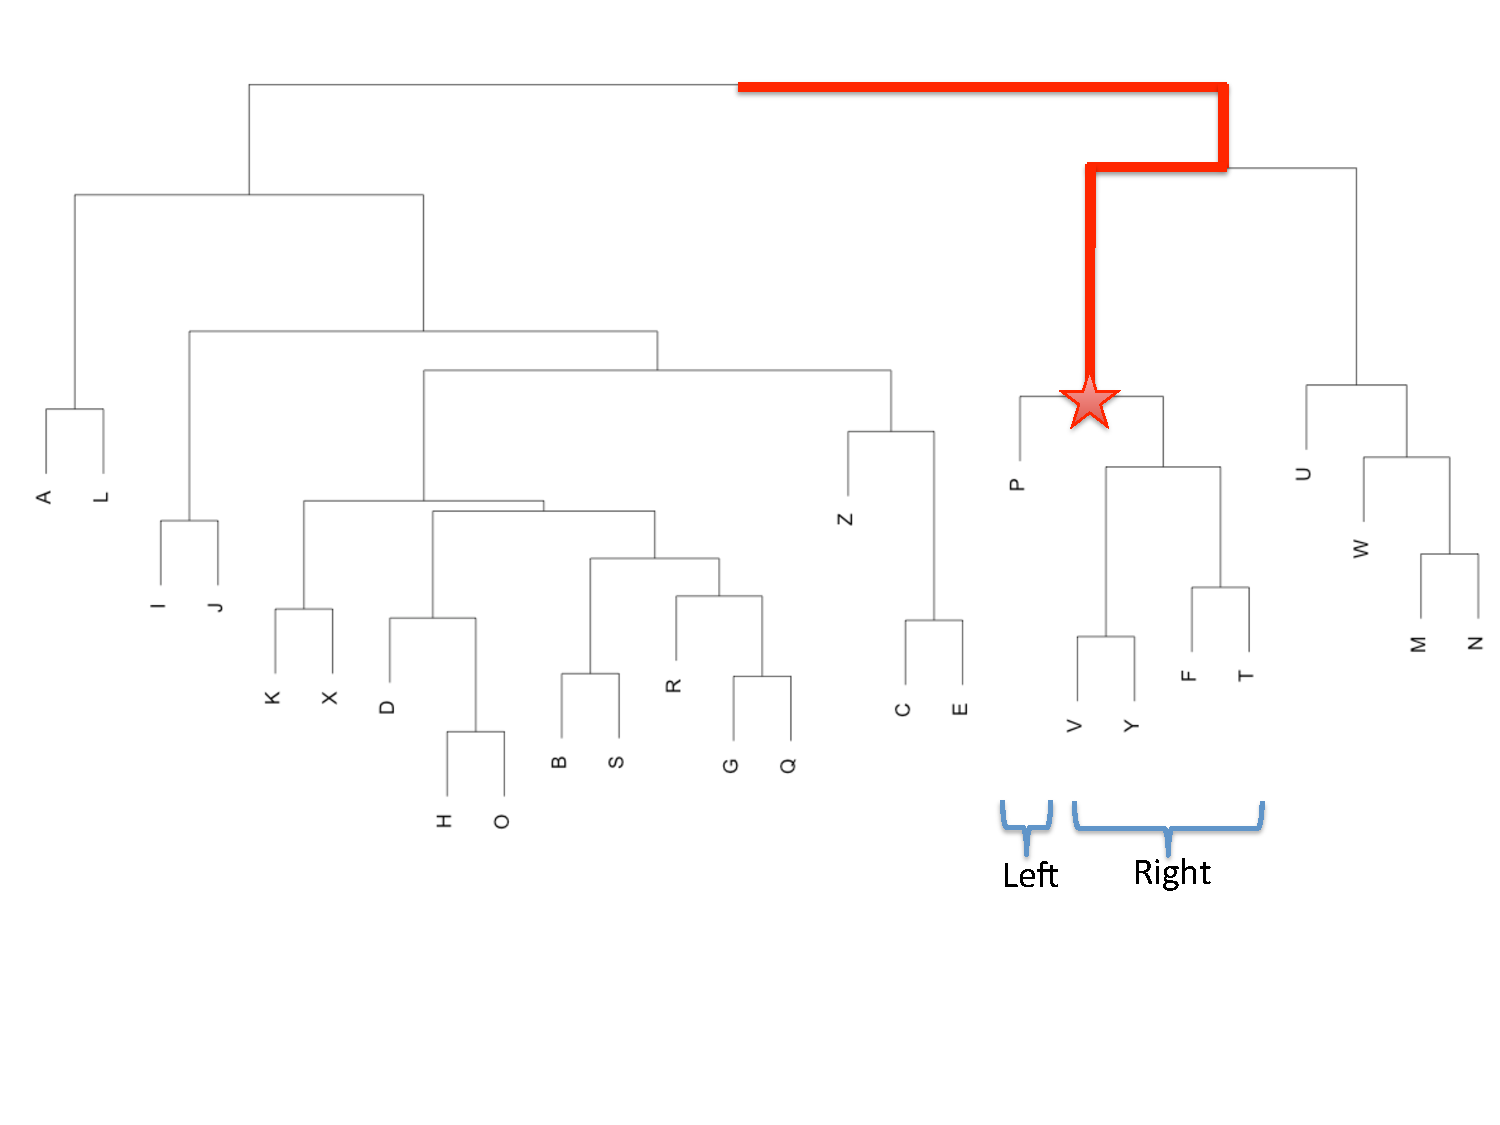
\includegraphics[width=.7 \textwidth]{thirdStep}

\tiny{$log(\frac{\pi_i}{1-\pi_i})= -23.41+.16x_1+.17x_2+.04x_3-.25x_4-.49x_5+.38x_6+.67x_7-.65x_8+.69x_{9}+.23x_{10}+.91x_{11}+1.79x_{12}+.36x_{13}-.1x_{14}+.07x_{15}-.29x_{16} \rightarrow \hat{\pi}=0.999$}
\end{center}
Move right!

\end{frame}


\begin{frame}
\frametitle{\small{Logistic Regression BST Algorithm Example}}
\small{New observation: ( T, 2,     6,     3,    4,     2,     7,    12,      2,      7,      7,      11,       8,     1,11,     1,      8)}
\begin{center} 
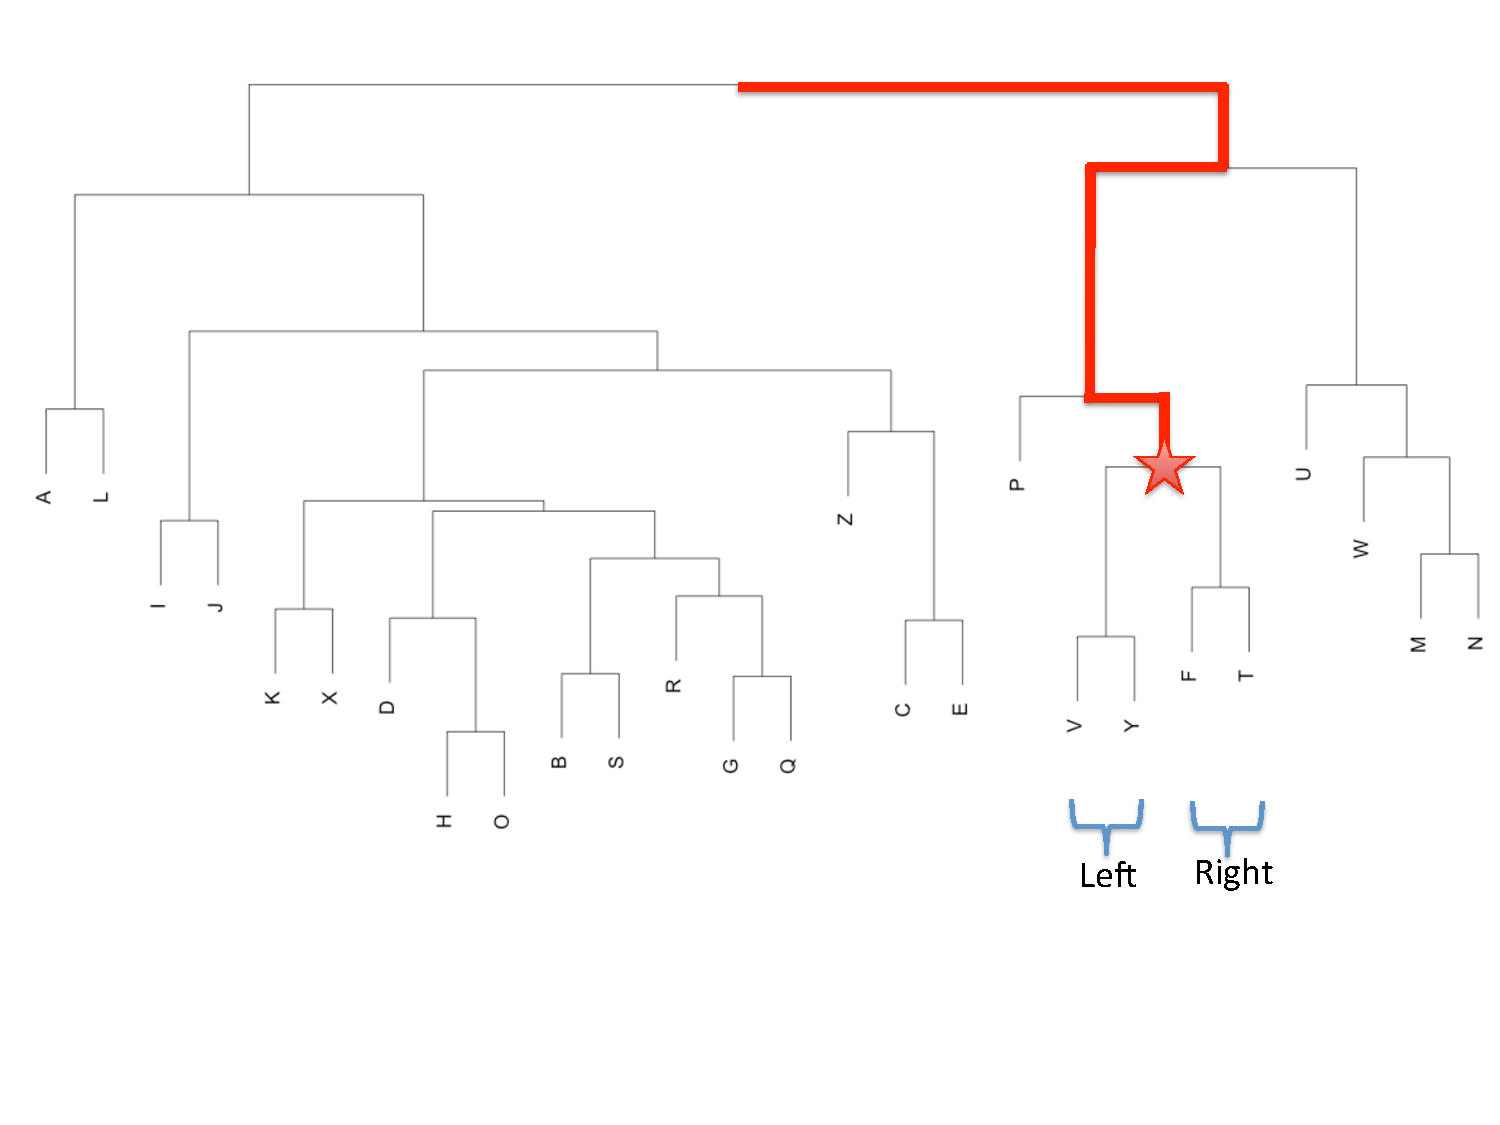
\includegraphics[width=.7 \textwidth]{fourthStep}

\tiny{$log(\frac{\pi_i}{1-\pi_i})= -13.86-.61x_1+.5x_2-.96x_3-.49x_4+1.57x_5+.57x_6+1.64x_7+.69x_8+1.56x_{9}+.85x_{10}-1.71x_{11}+.32x_{12}-.65x_{13}-.96x_{14}-.55x_{15}+.58x_{16} \rightarrow \hat{\pi}=0.991$}
\end{center}
Move right!

\end{frame}

\begin{frame}
\frametitle{\small{Logistic Regression BST Algorithm Example}}
\small{New observation: ( T, 2,     6,     3,    4,     2,     7,    12,      2,      7,      7,      11,       8,     1,11,     1,      8)}
\begin{center} 
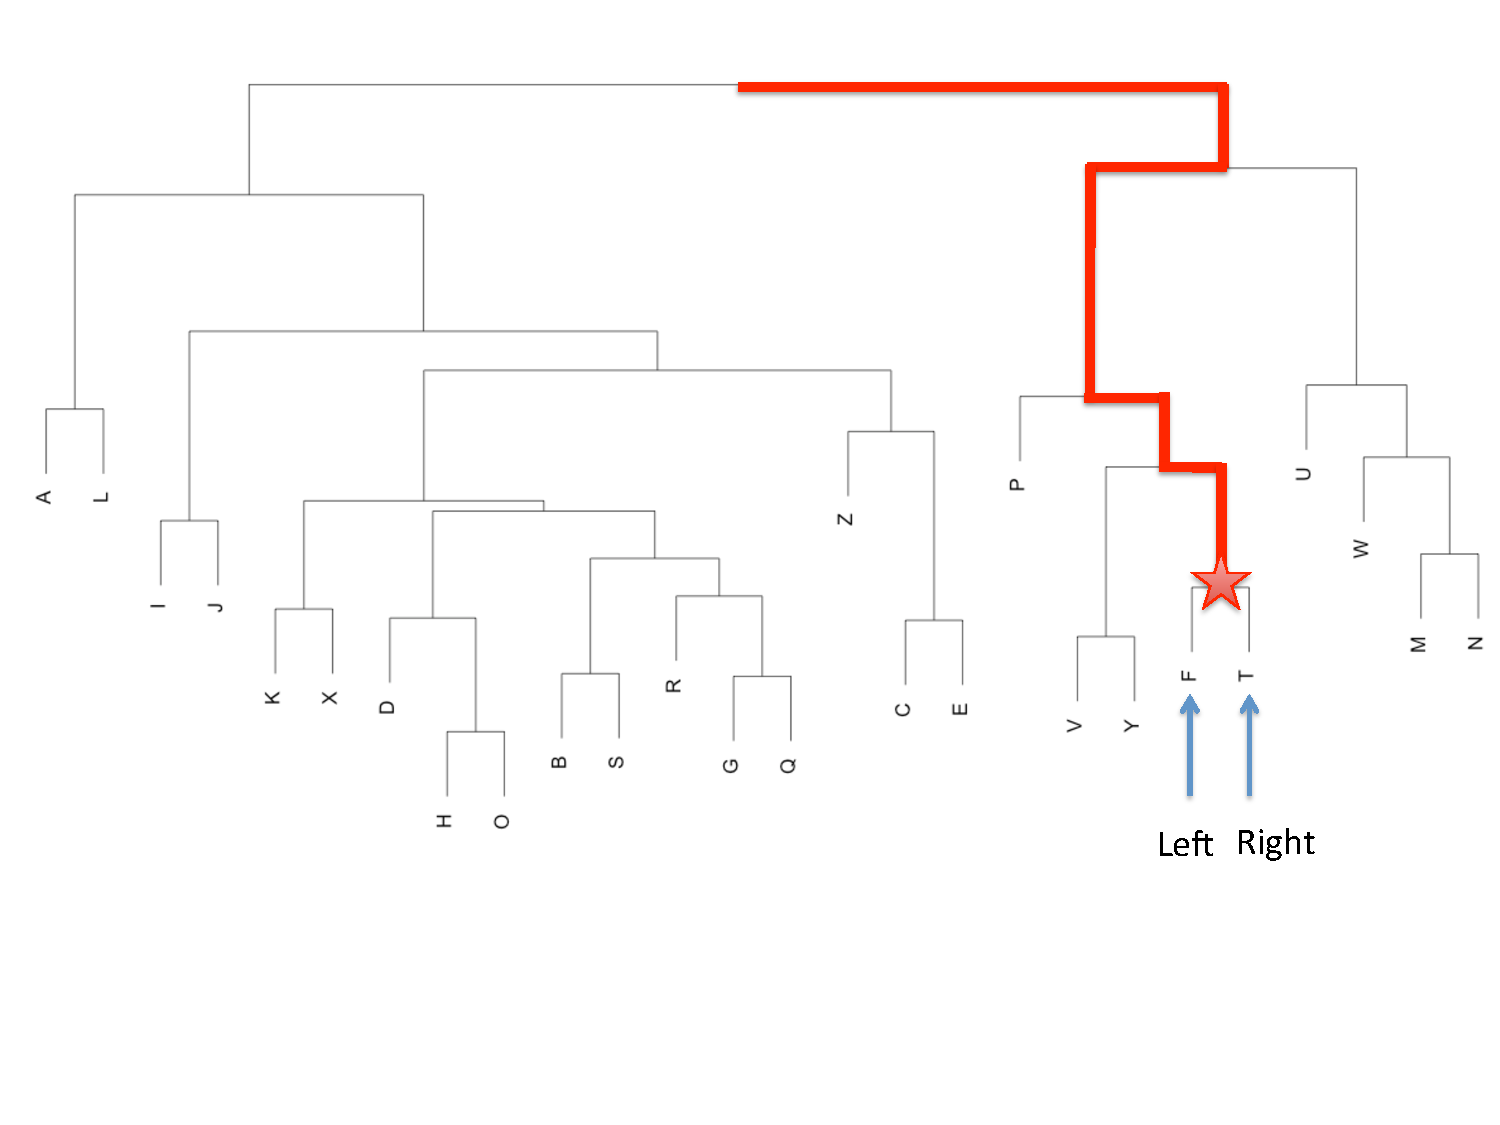
\includegraphics[width=.7 \textwidth]{fifthStep}

\tiny{$log(\frac{\pi_i}{1-\pi_i})= -33.85+.99x_1+.77x_2-.59x_3-1.36x_4-.04x_5+1.5x_6+2.41x_7+1.22x_8+3.35x_{9}-1.96x_{10}-.87x_{11}+1.61x_{12}+.33x_{13}+.66x_{14}-1.25x_{15}-1.32x_{16} \rightarrow \hat{\pi}=0.999$}
\end{center}
Move right! and STOP

\end{frame}

\begin{frame}
\frametitle{\small{Logistic Regression BST Algorithm Example}}
\small{New observation: ( T, 2,     6,     3,    4,     2,     7,    12,      2,      7,      7,      11,       8,     1,11,     1,      8)}
\begin{center} 
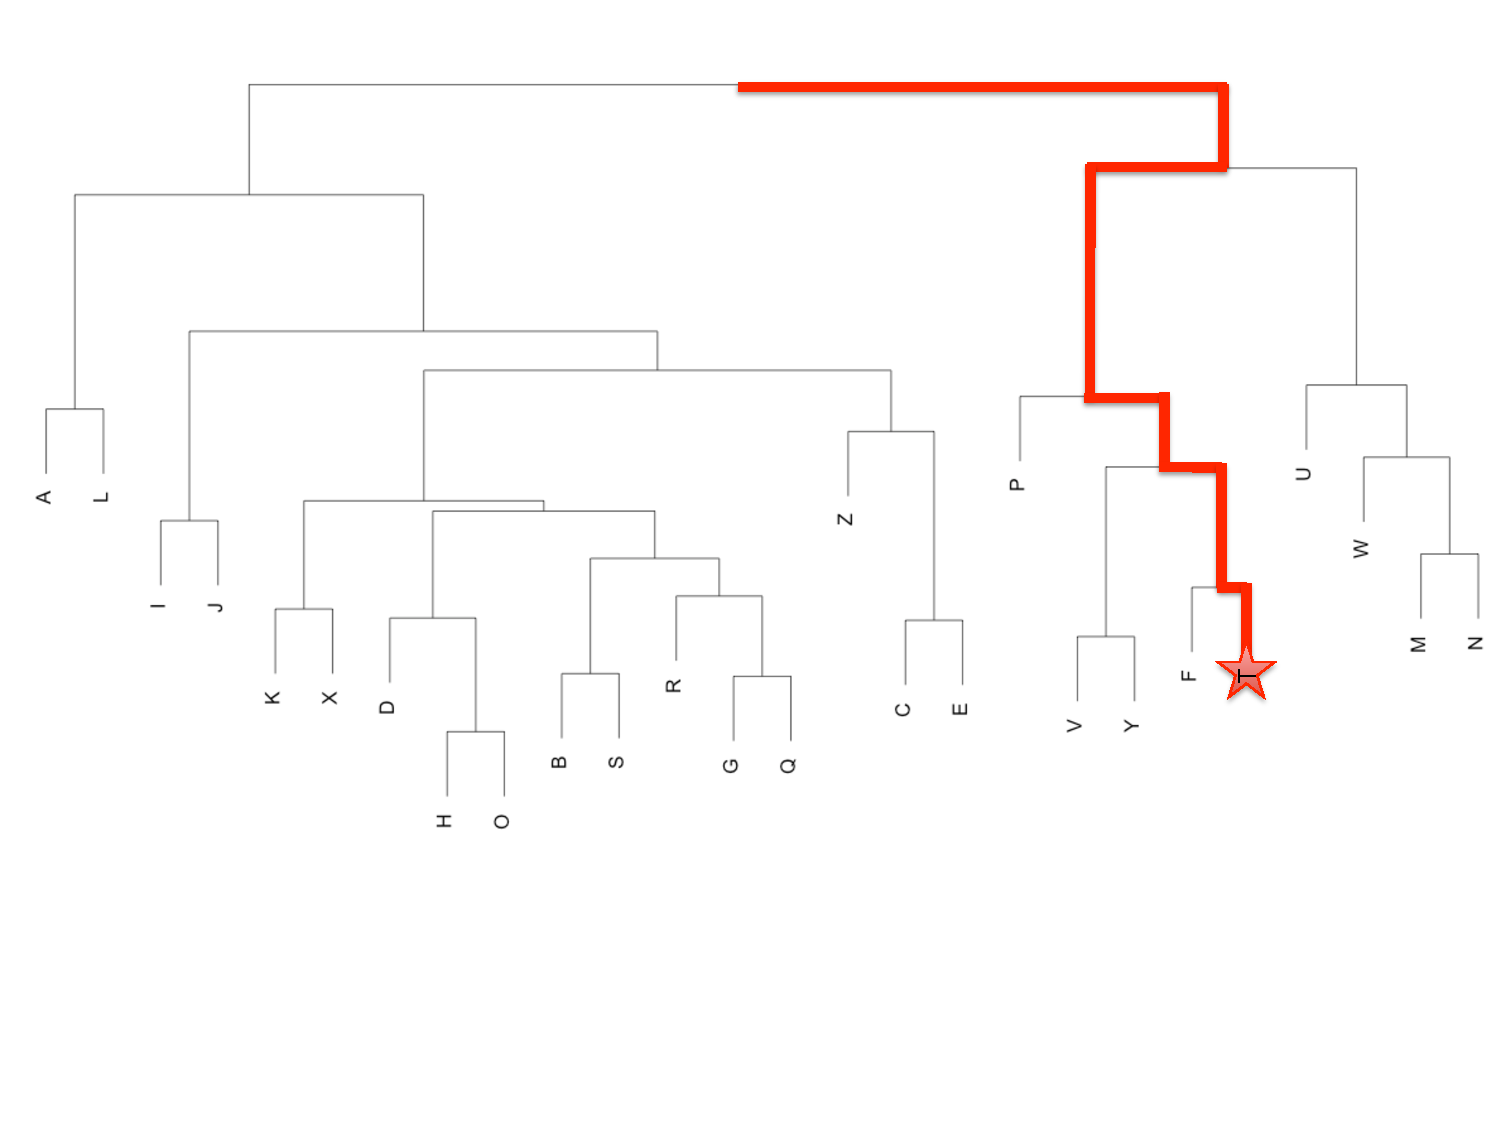
\includegraphics[width=.7 \textwidth]{sixthStep}

\end{center}

Prediction: T 

Conclusion: Correctly classified! Yay!

\end{frame}

\subsection{Decision Tree Algorithm}
\begin{frame}
\frametitle{Decision Tree Algorithm}
Constructing Decision Tree (Using Learning Set):
\begin{enumerate}
\item \small{All training set observations are lumped into a single node}
\item \small{The majority class - which class of letter has the most observations in the active node - is identified.}
\item \small{The Gini index is calculated for the active node.}
\begin{enumerate}
\item \small{For every covariate at every possible splt point the Gini index is calculated for the two new created nodes after the considered splot.}
\item \small{A weighted average is taken on the two indices.}
\item \small{The coviariate/split point combination that produces the largest (Original Gini Index - Sum(Split Gini Indices)) is chosen as the split criteria.}
\end{enumerate}
\item \small{The split is created creating two new nodes.}
\item \small{Steps 2 through 4 are repeated for each new node, up to a certain threshold.}
\end{enumerate}
\end{frame}

\begin{frame}
\frametitle{What is a Gini Impurity Index (GII)?}
\begin{itemize}
\item The Gini index is a number that represents the "impurity" in a node, i.e. the amount of mixing of classes present
\item A pure node would be one consisting of only a single class, then Gini index = 0
\item A node with equal amounts of every class would be perfectly impure, and the Gini would be at maximum (no upper bound)
\end{itemize}
\end{frame}

\begin{frame}
\frametitle{Traversing Decision Tree}
\begin{enumerate}
\item A new observation is introduced.
\item The first decision point - i.e., split point/covariate combination - is reached. If the covariate for the new observation is less than the split point, it goes left; if it is greater, it goes right.
\item Step 1 is repeated until a terminal node is reached, and a class is assigned.
\end{enumerate}
\end{frame}



\begin{frame}
\frametitle{Full CART Decision Tree}
\begin{center} 
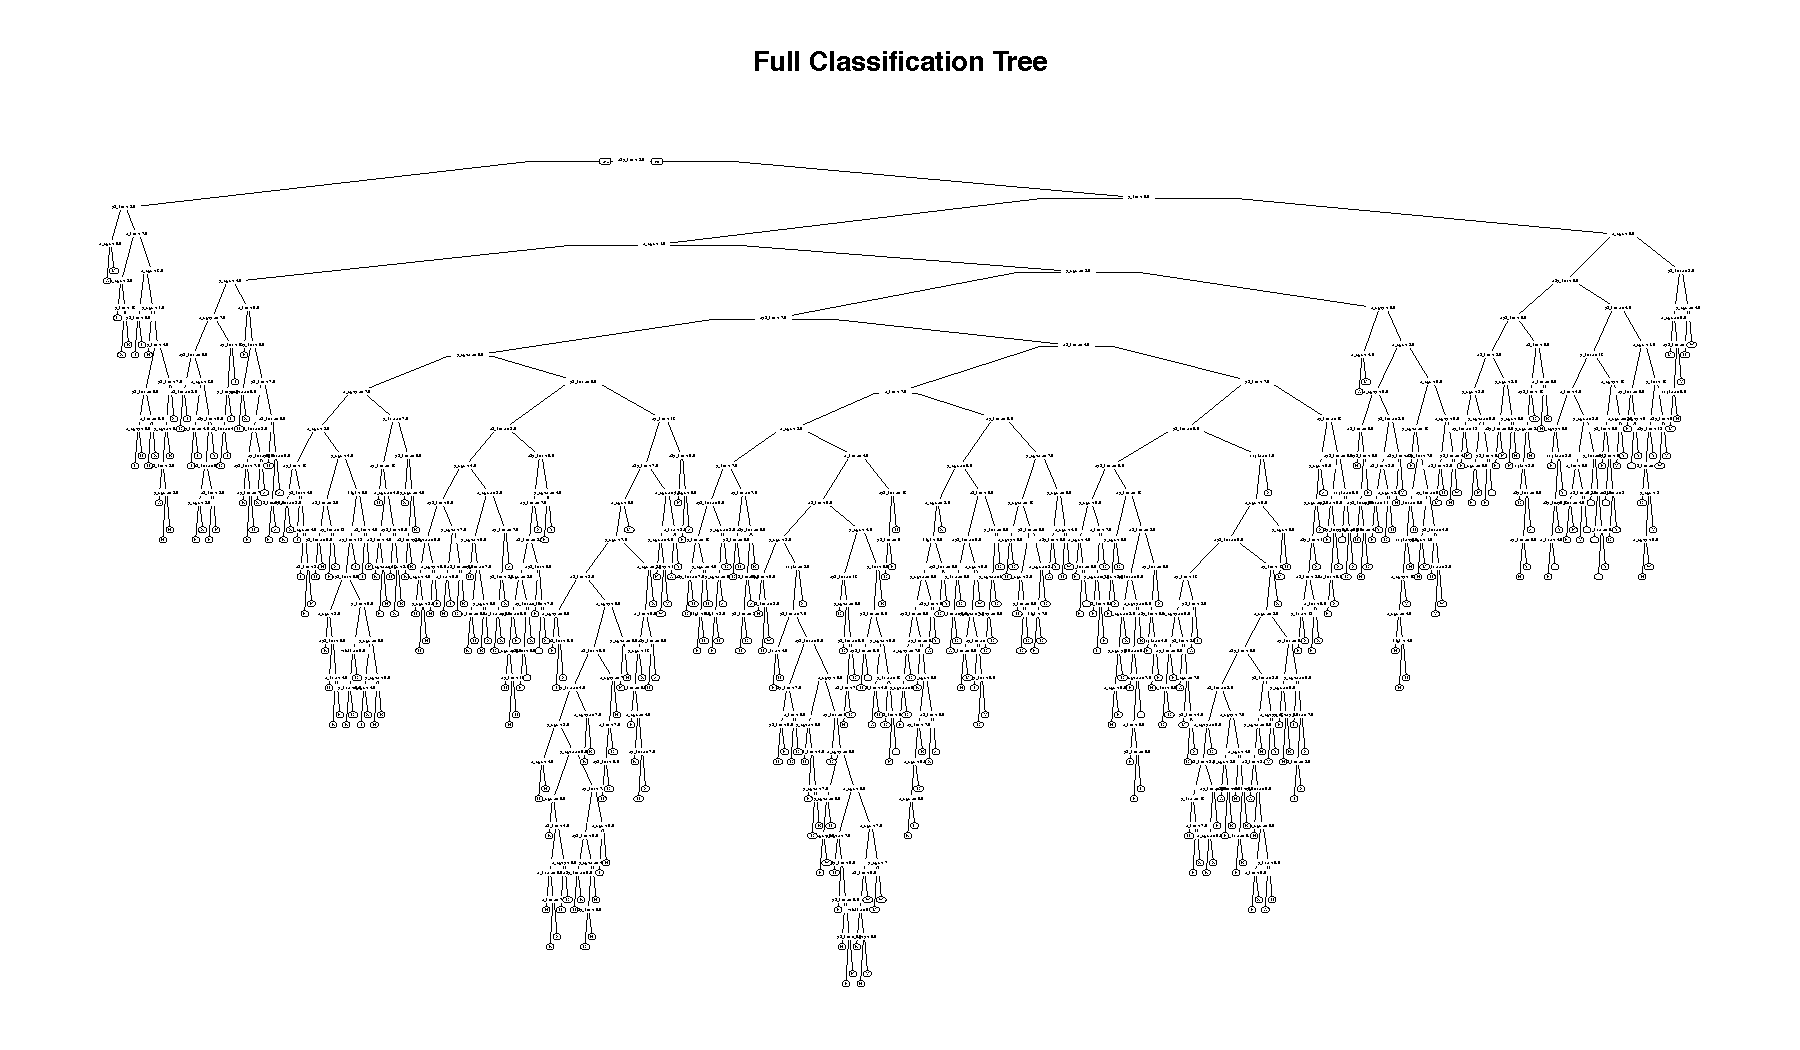
\includegraphics[width=1 \textwidth]{FullCT}
\end{center}

\end{frame}

\begin{frame}
\frametitle{Full CART Decision Tree Zoom In }
\begin{center} 
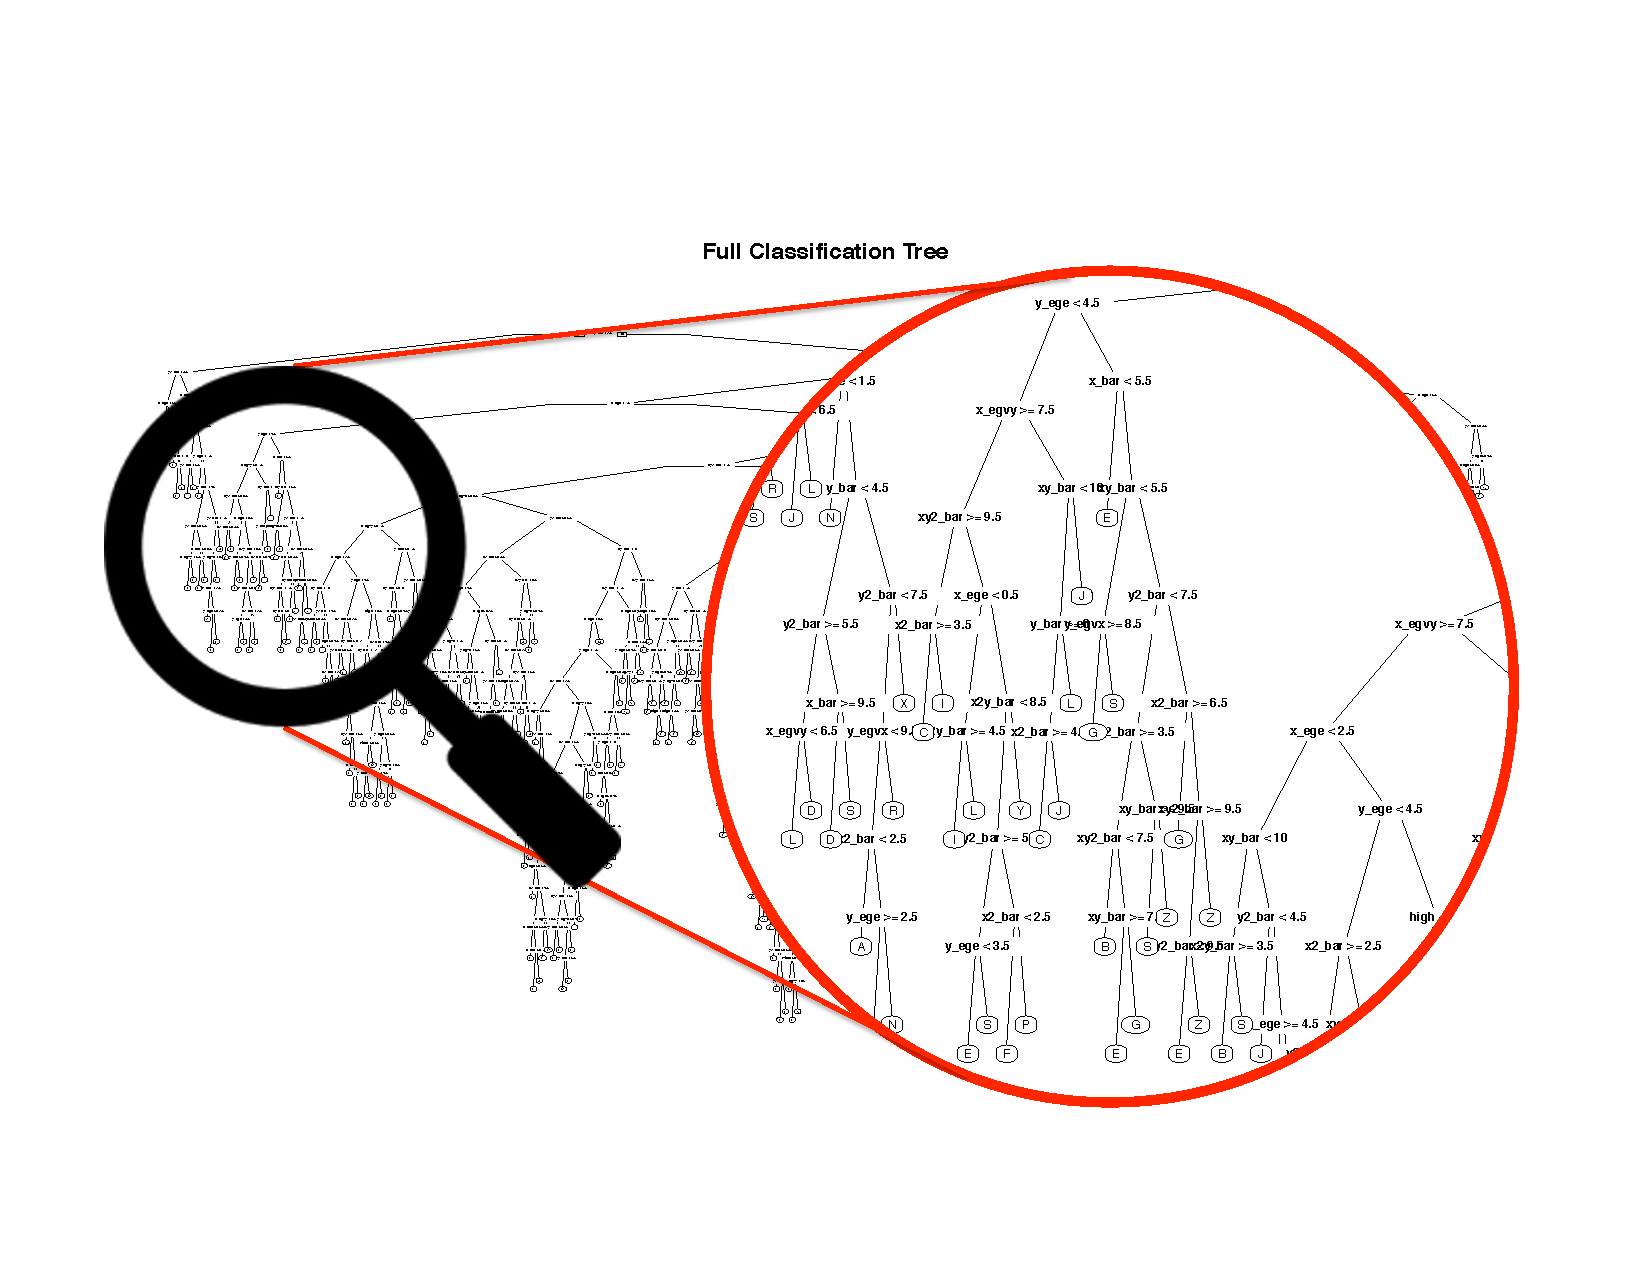
\includegraphics[width=.8 \textwidth]{magGlass}

\small{After tree is created it requires "pruning" to get rid of repeated nodes.}
\end{center}
\end{frame}

\begin{frame}
\frametitle{How should we prune?}
\begin{center} 
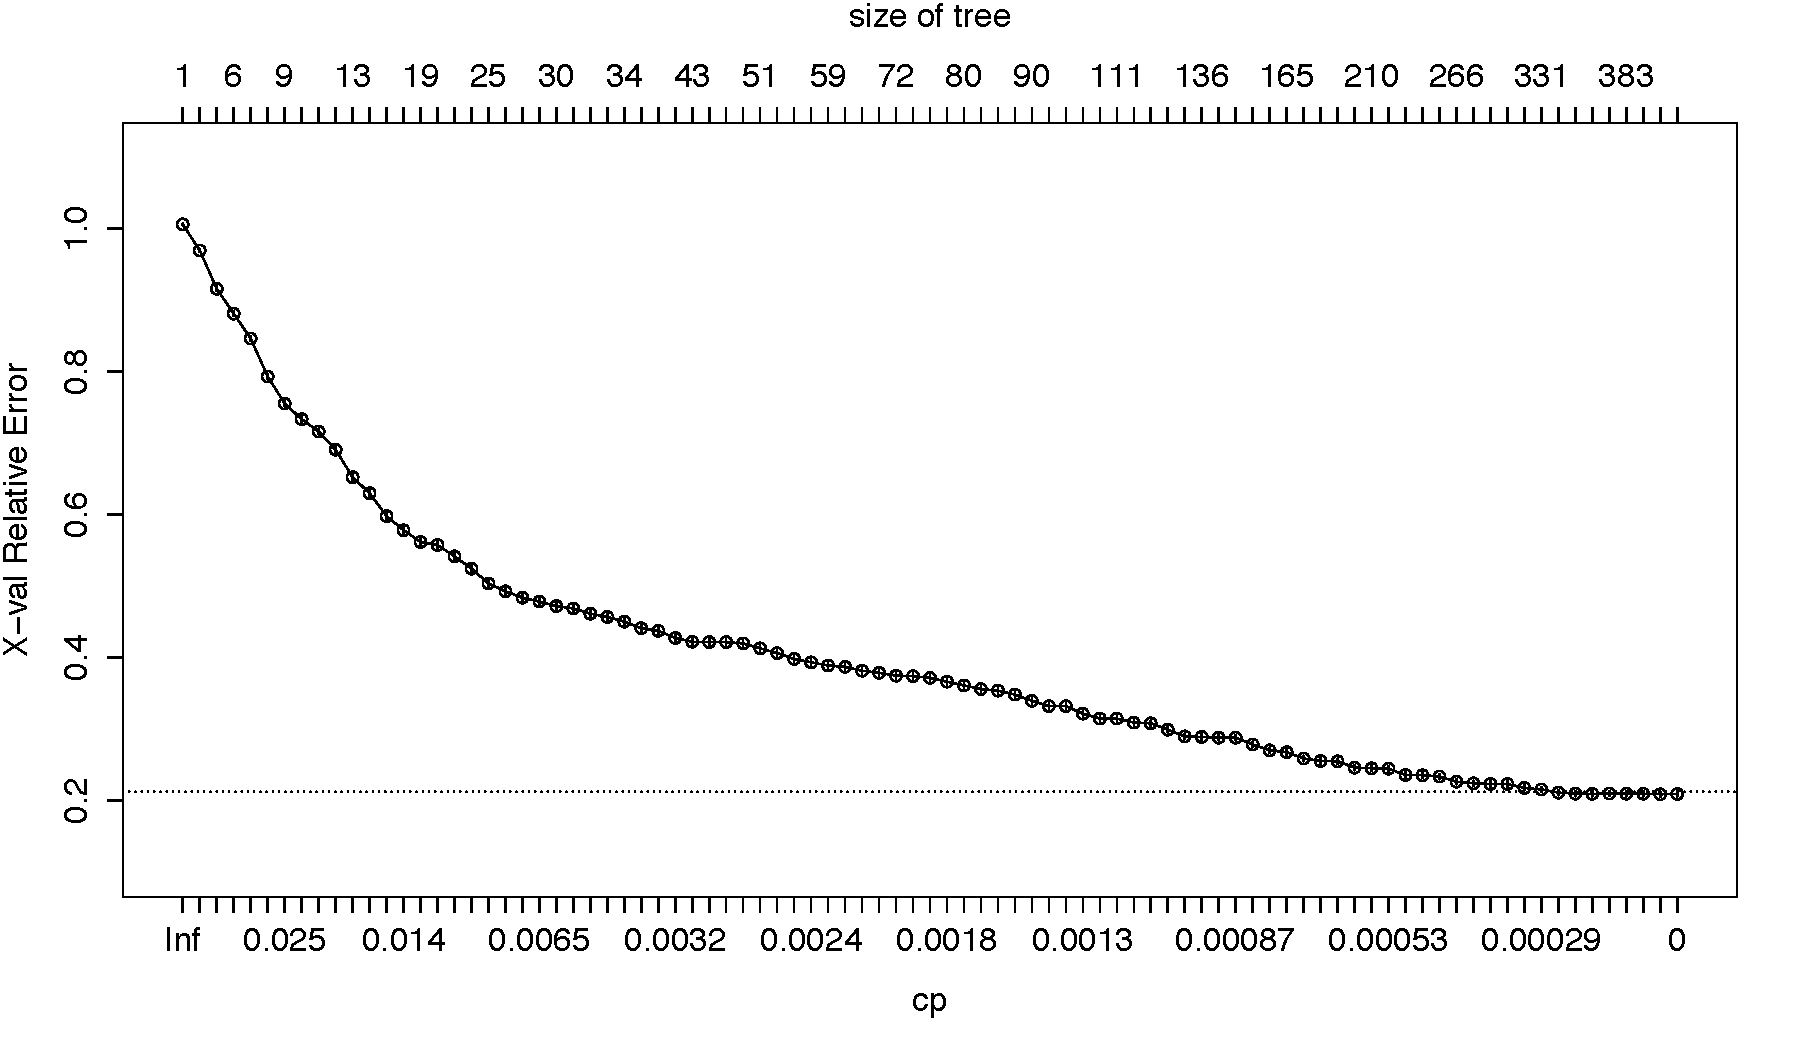
\includegraphics[width=1 \textwidth]{cpPlot}
\end{center}

\end{frame}

\begin{frame}
\frametitle{Pruned CART Decision Tree}
\begin{center} 
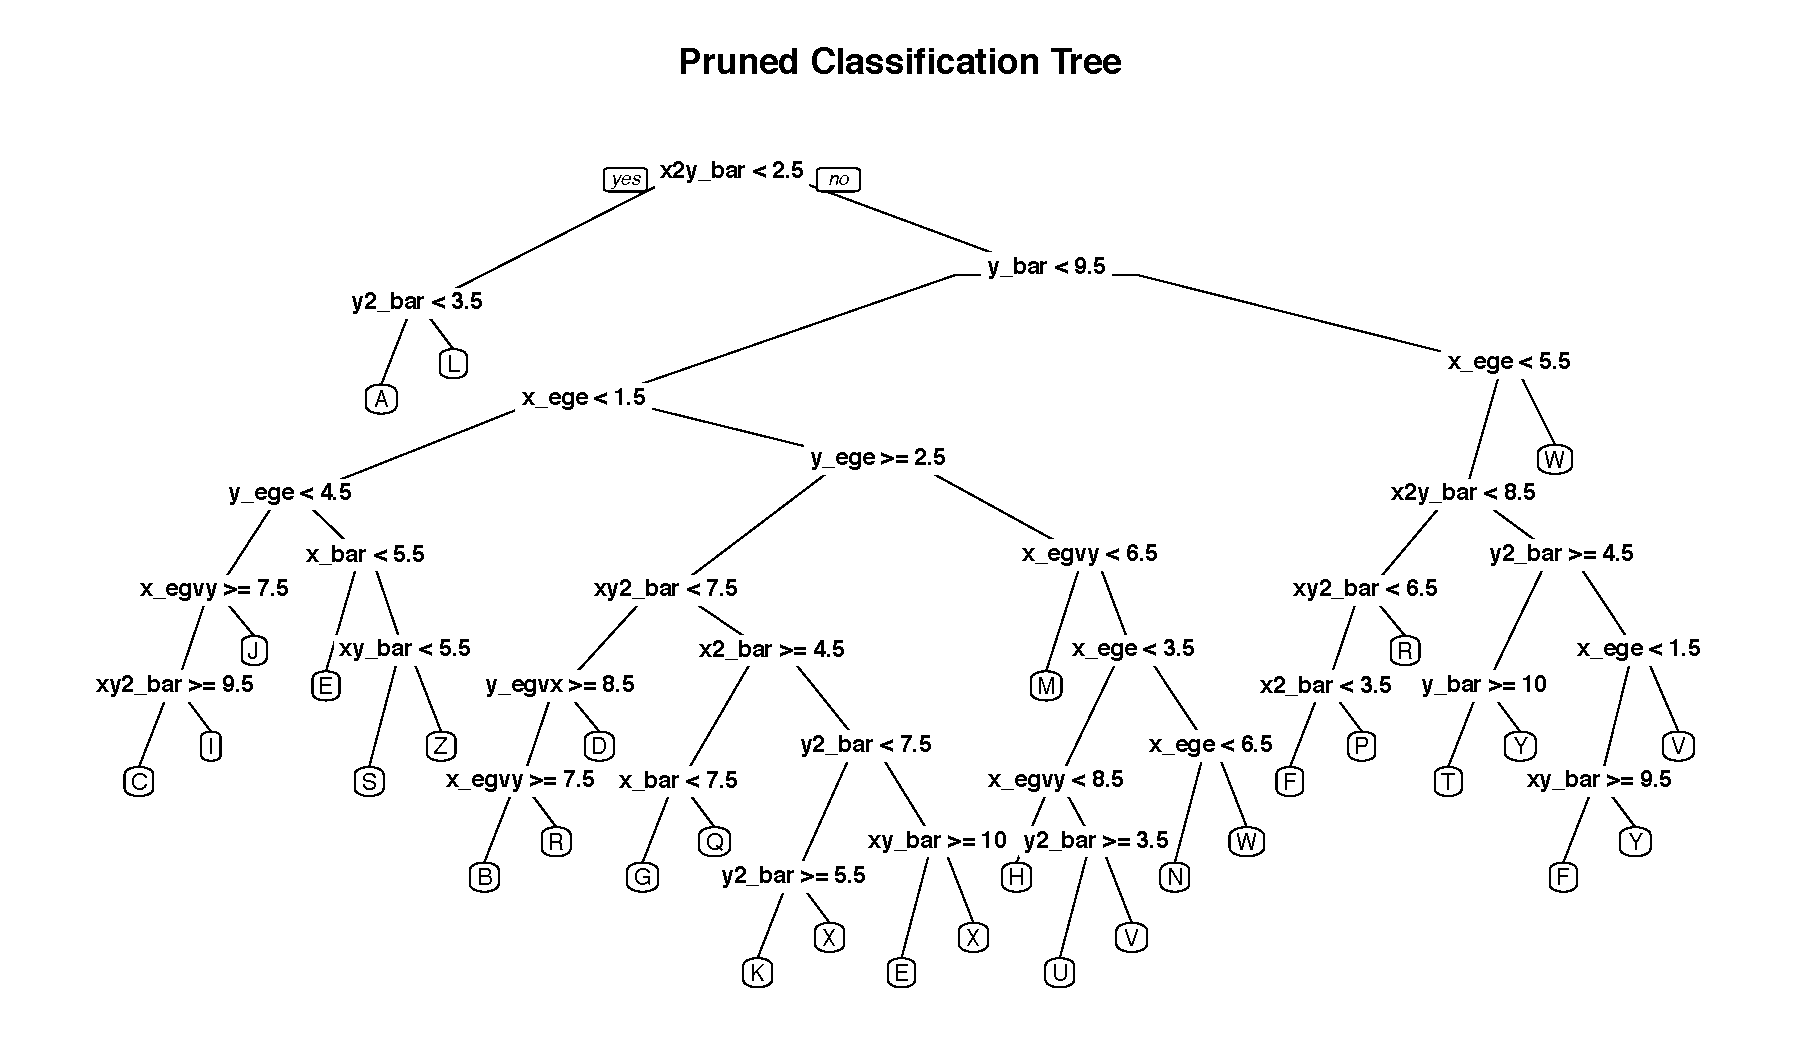
\includegraphics[width=1 \textwidth]{PrunedCT}
\end{center}
\end{frame}

\begin{frame}
\frametitle{CART vs BAG Methods}
\begin{itemize}
\item CART model is based on using a single tree for each of the predictions made.  
\begin{itemize}
\item Fails to classify 7 classes
\end{itemize}
\item BAG model is based on aggregation (bootstrap) of votes from all the trees used in the model.  
\begin{itemize}
\item performs better (it predicts all classes, even if not perfectly)
\end{itemize}
\end{itemize}

\end{frame}

\begin{frame}
\frametitle{Bagging Error Plot}
\begin{center} 
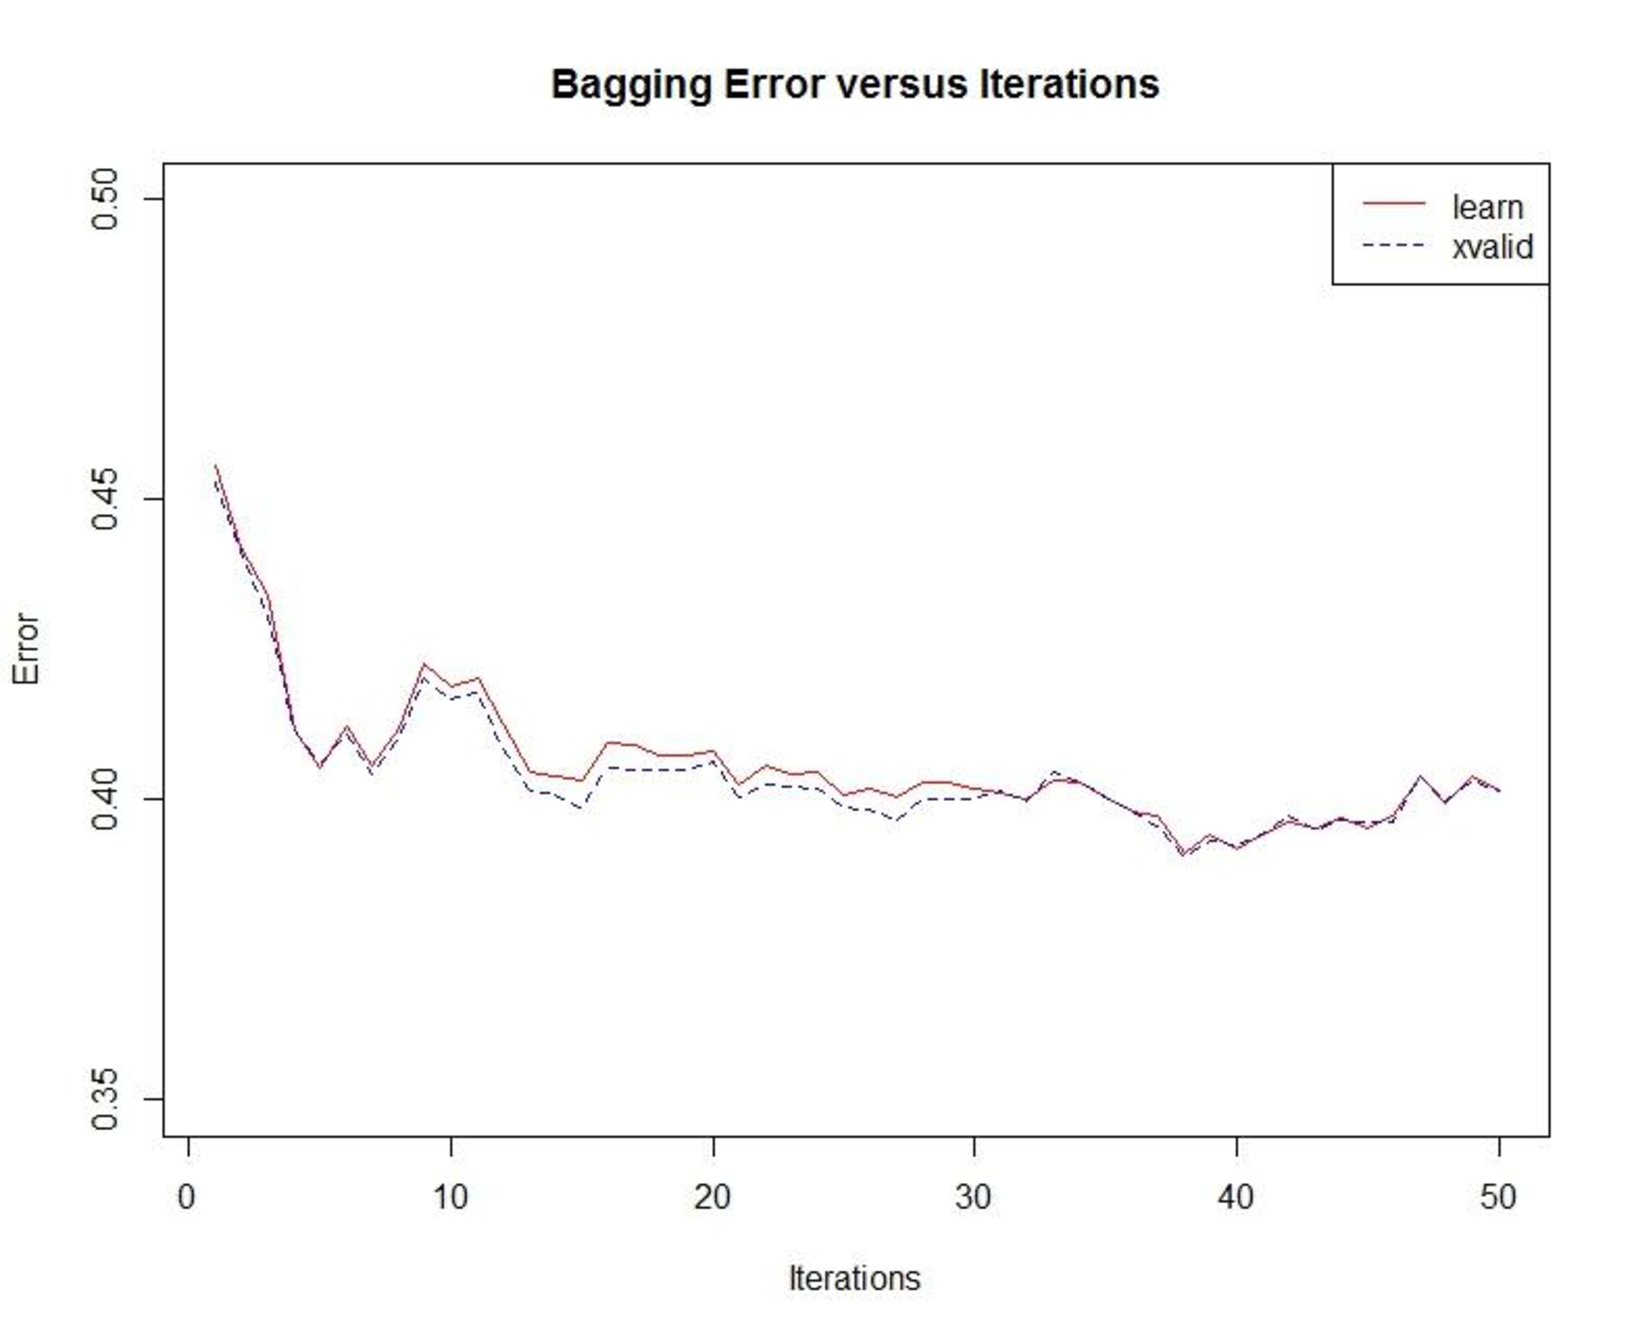
\includegraphics[width=.6 \textwidth]{bagErr}
\end{center}
\end{frame}



\section{Summary of Findings}
\begin{frame}
\frametitle{Summary of Findings}
Findings for: 
\begin{enumerate}
\item Logistic Regression BST Confusion Matrix
\item Decision Trees for Classification
\begin{enumerate}
\item CART Method Confusion Matrix
\item Bag Method Confusion Matrix
\end{enumerate}
\end{enumerate}
\end{frame}

\begin{frame}
\frametitle{Overall Findings}
\begin{enumerate}
\item Logistic Regression BST : $74.8\%$ Correct Specification Overall
\begin{itemize}
\item Highest Correct Classification: \textbf{W} with $94\%$
\item Lowest Correct Classification: \textbf{H} with $40\%$
\end{itemize}
\item CART Method: $47.1\%$ Correct Specification Overall
\begin{itemize}
\item Highest Correct Classification: \textbf{I} with $78\%$
\item Lowest Correct Classification: \textbf{E,F,K,O,R,S,Y} with $0\%$
\end{itemize}
\item Bag Method: $60.6\%$ Correct Specification Overall
\begin{itemize}
\item Highest Correct Classification: \textbf{V} with $82\%$
\item Lowest Correct Classification: \textbf{S} with $22\%$
\end{itemize}
\end{enumerate}
\end{frame}

\begin{frame}
\frametitle{Logistic Regression BST Distribution of Specification}
\begin{center} 
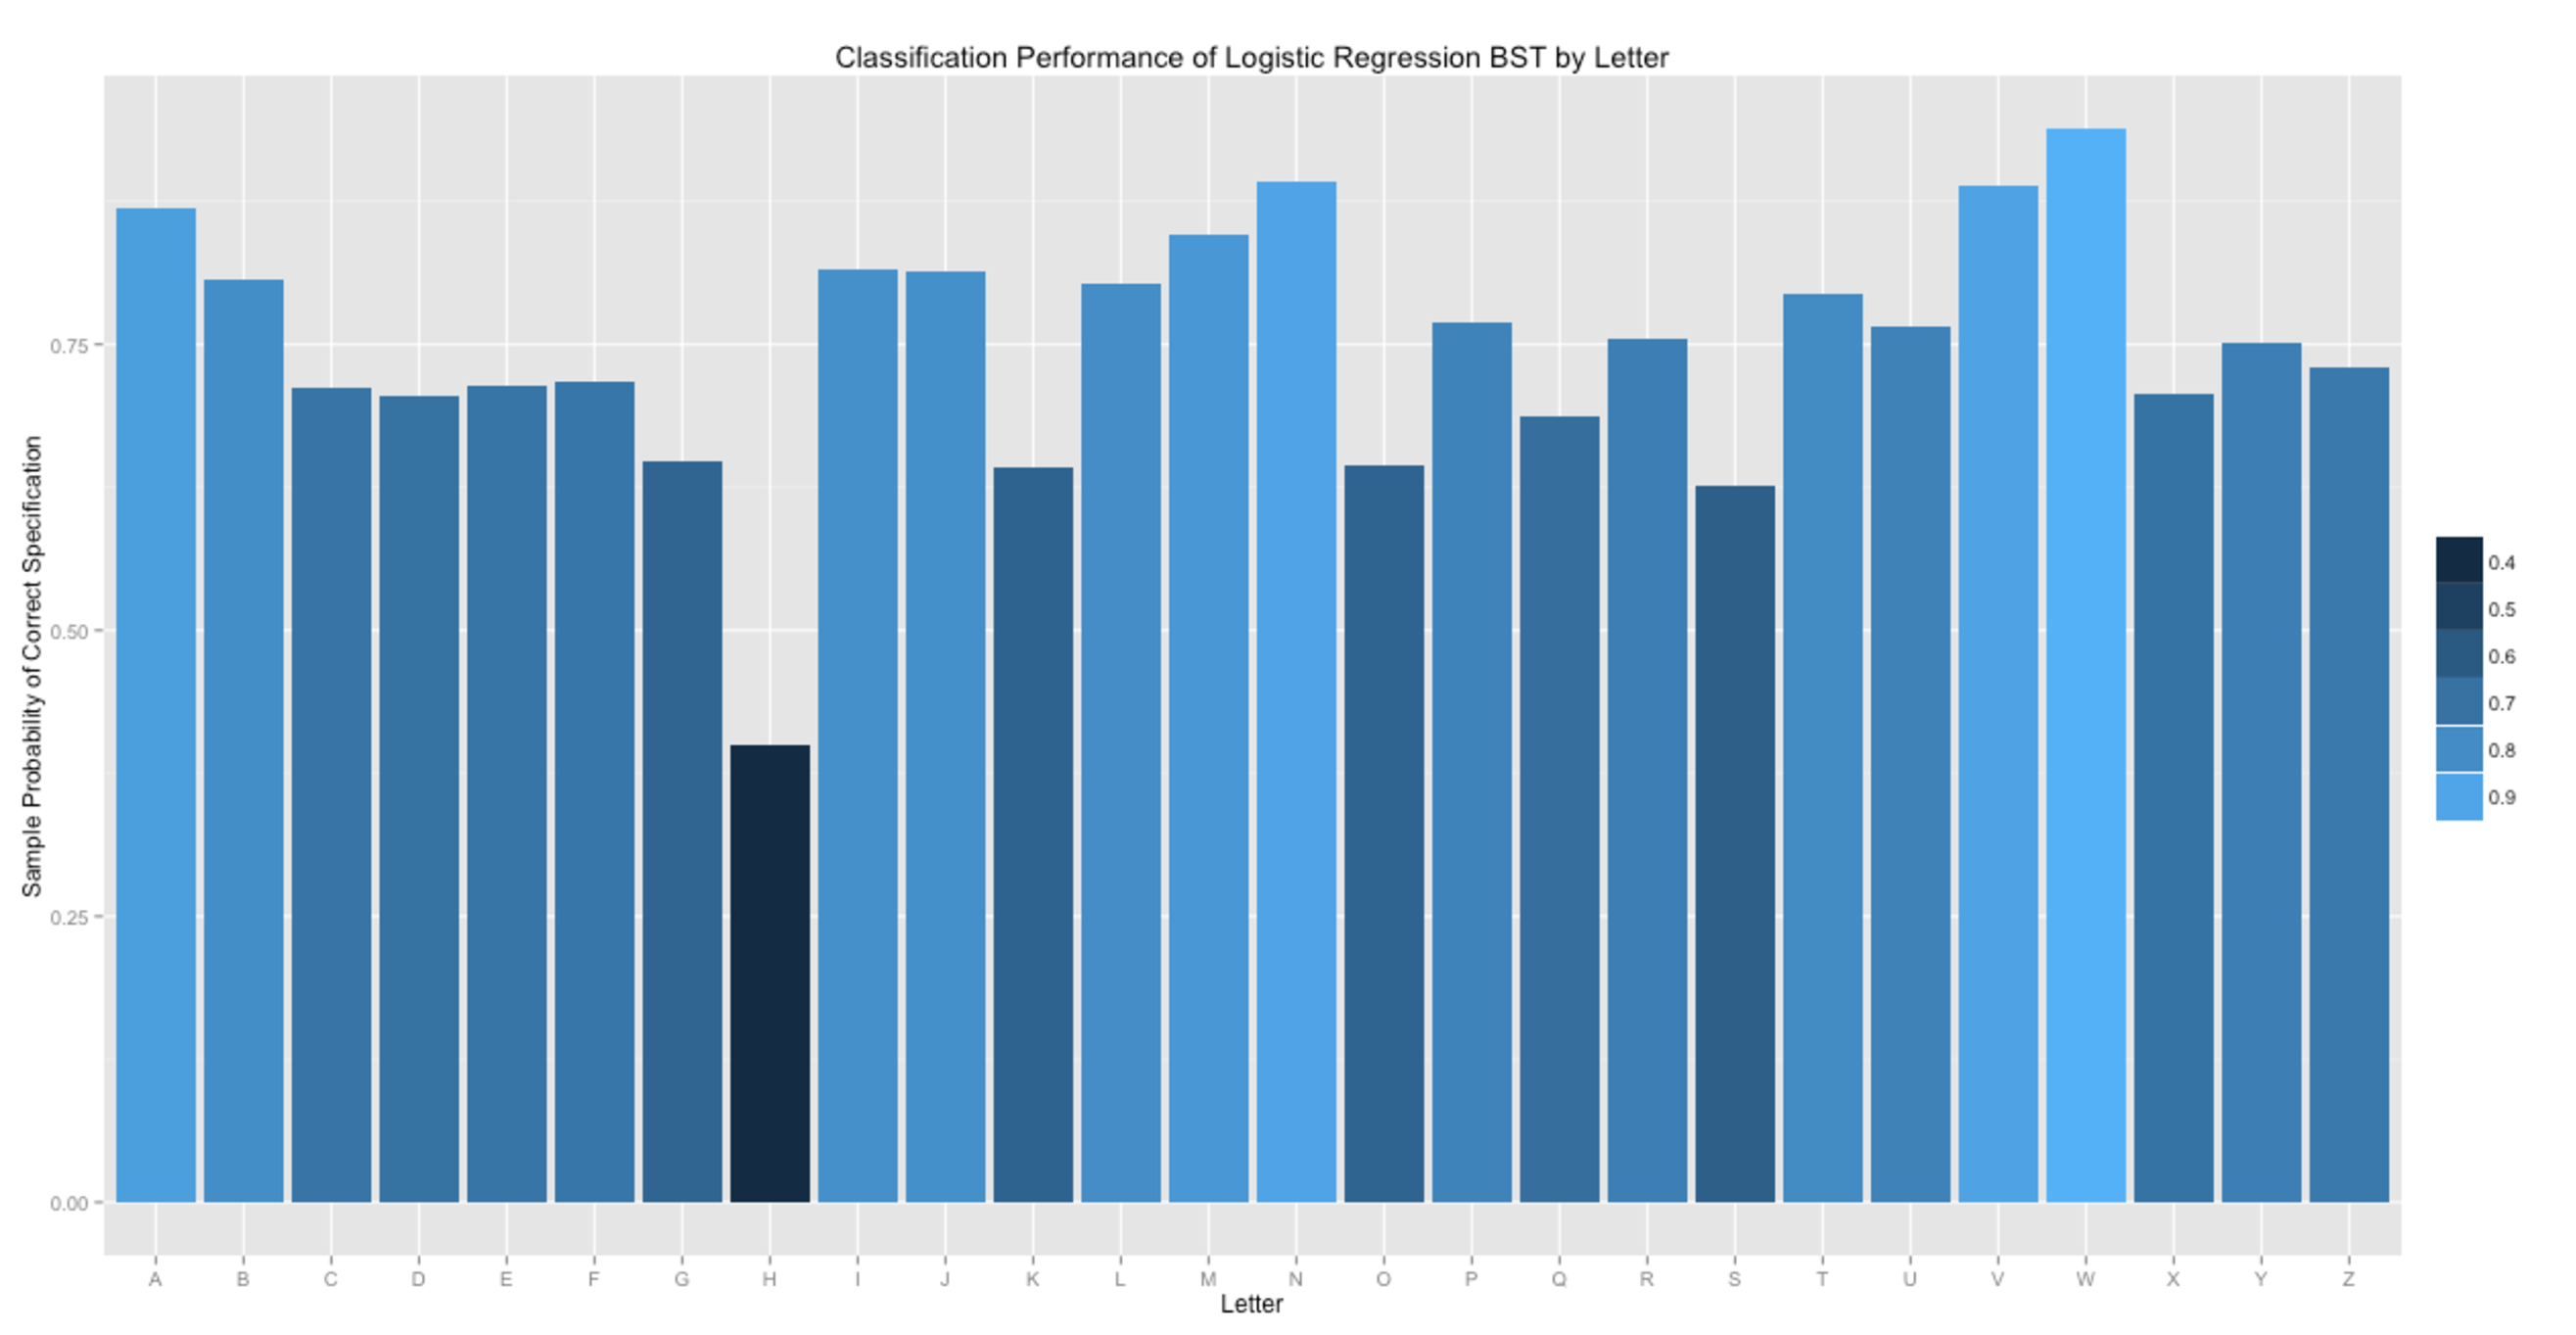
\includegraphics[width=1 \textwidth]{hkMiss}
\end{center}
\end{frame}


\begin{frame}
\frametitle{Logistic Regression BST Confusion Matrix}
\begin{center} 
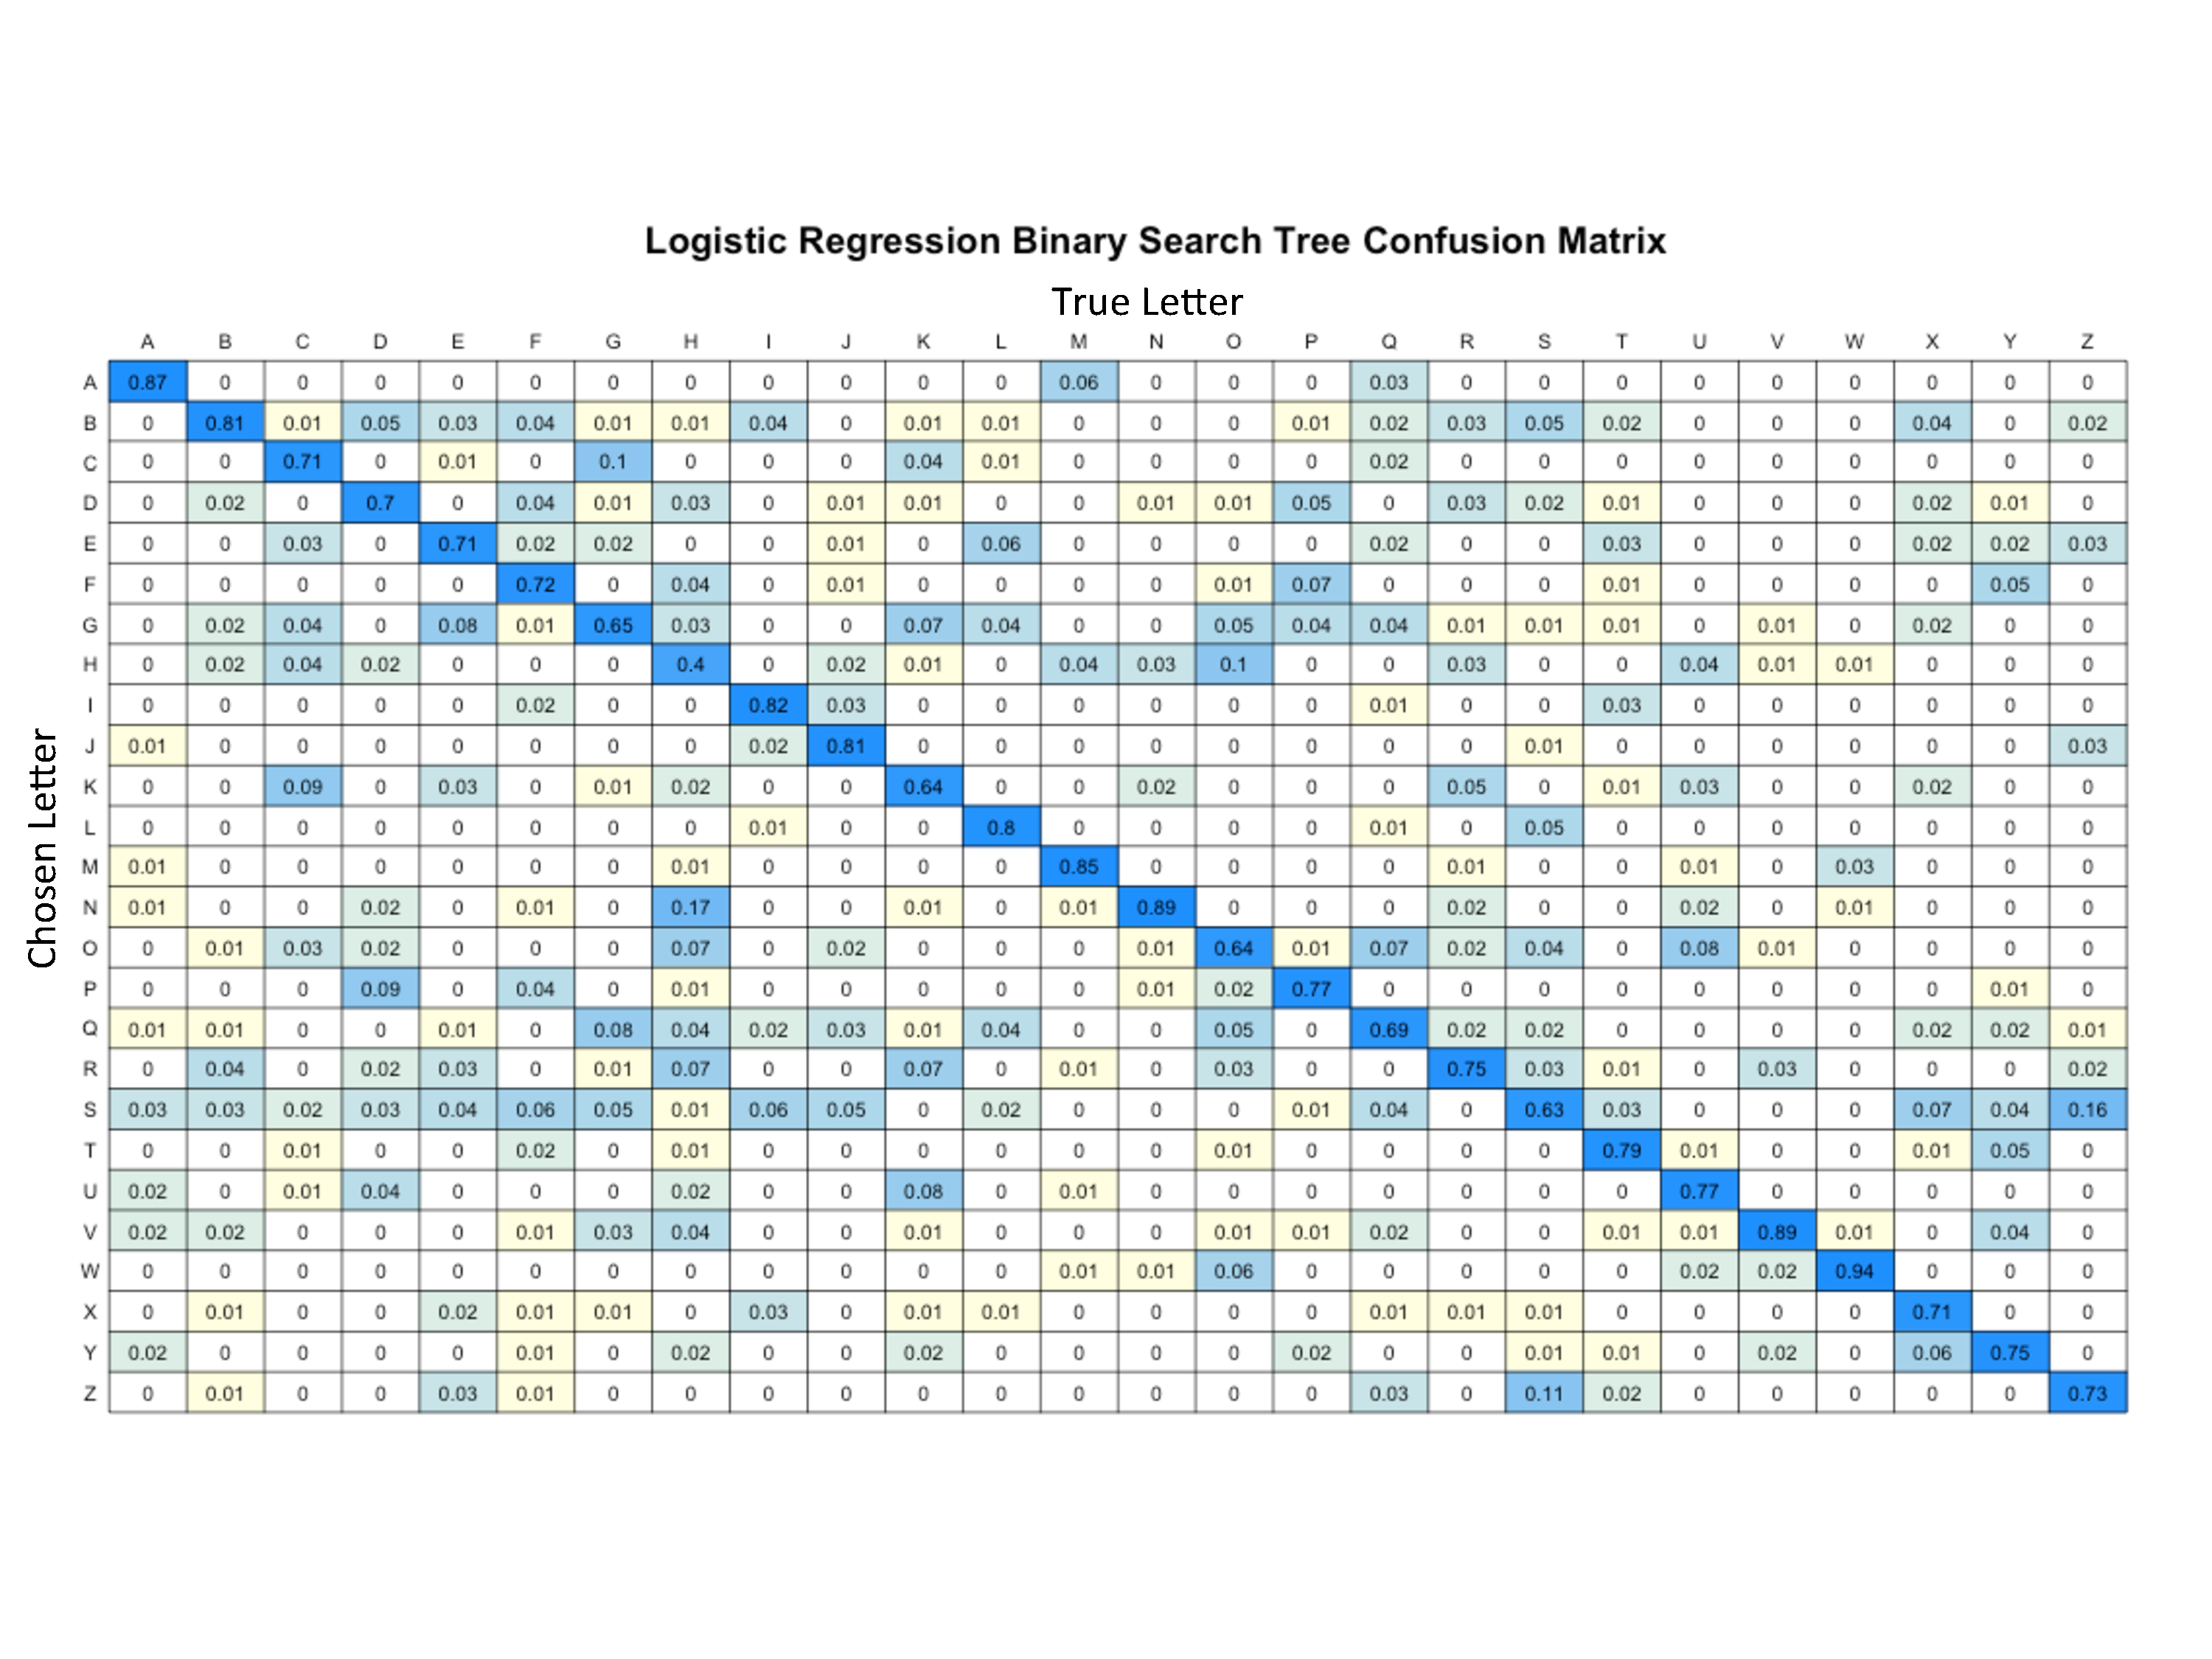
\includegraphics[width=1 \textwidth]{hkPercent}
\end{center}
\end{frame}

\begin{frame}
\frametitle{CART Method Distribution of Specification}
\begin{center} 
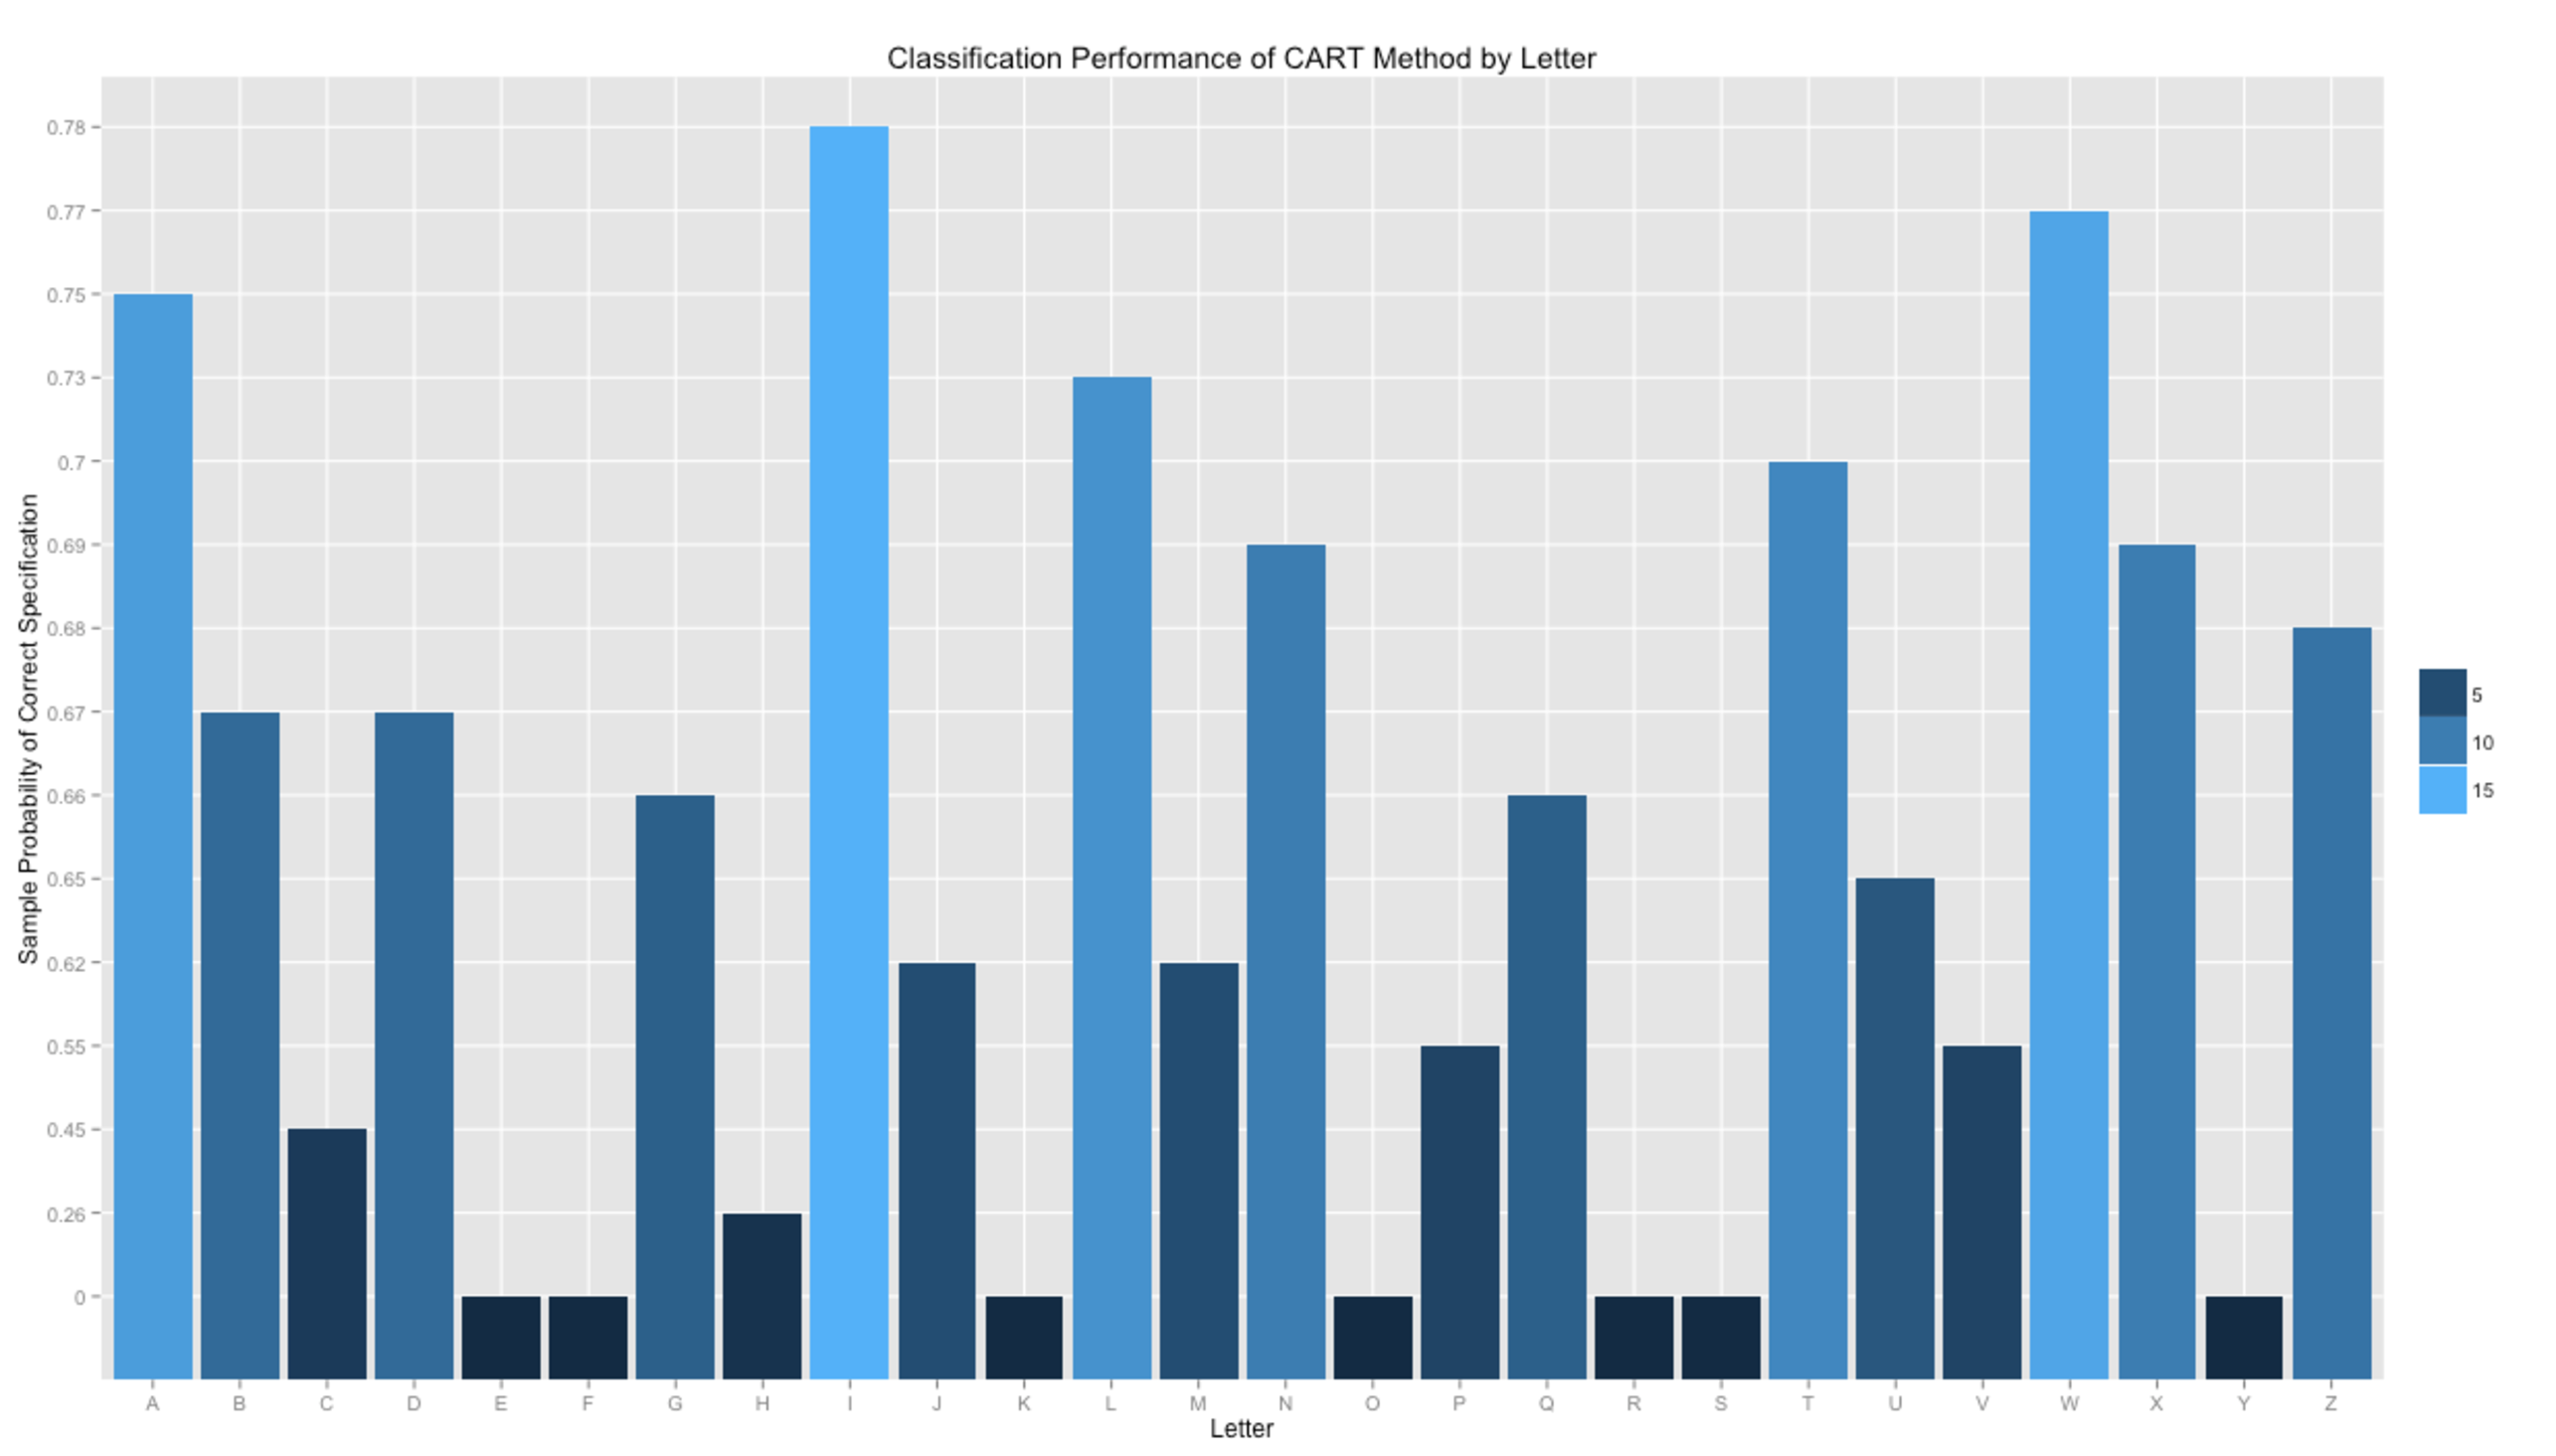
\includegraphics[width=1 \textwidth]{cartPlot}
\end{center}
\end{frame}


\begin{frame}
\frametitle{CART Method Confusion Matrix}
\begin{center} 
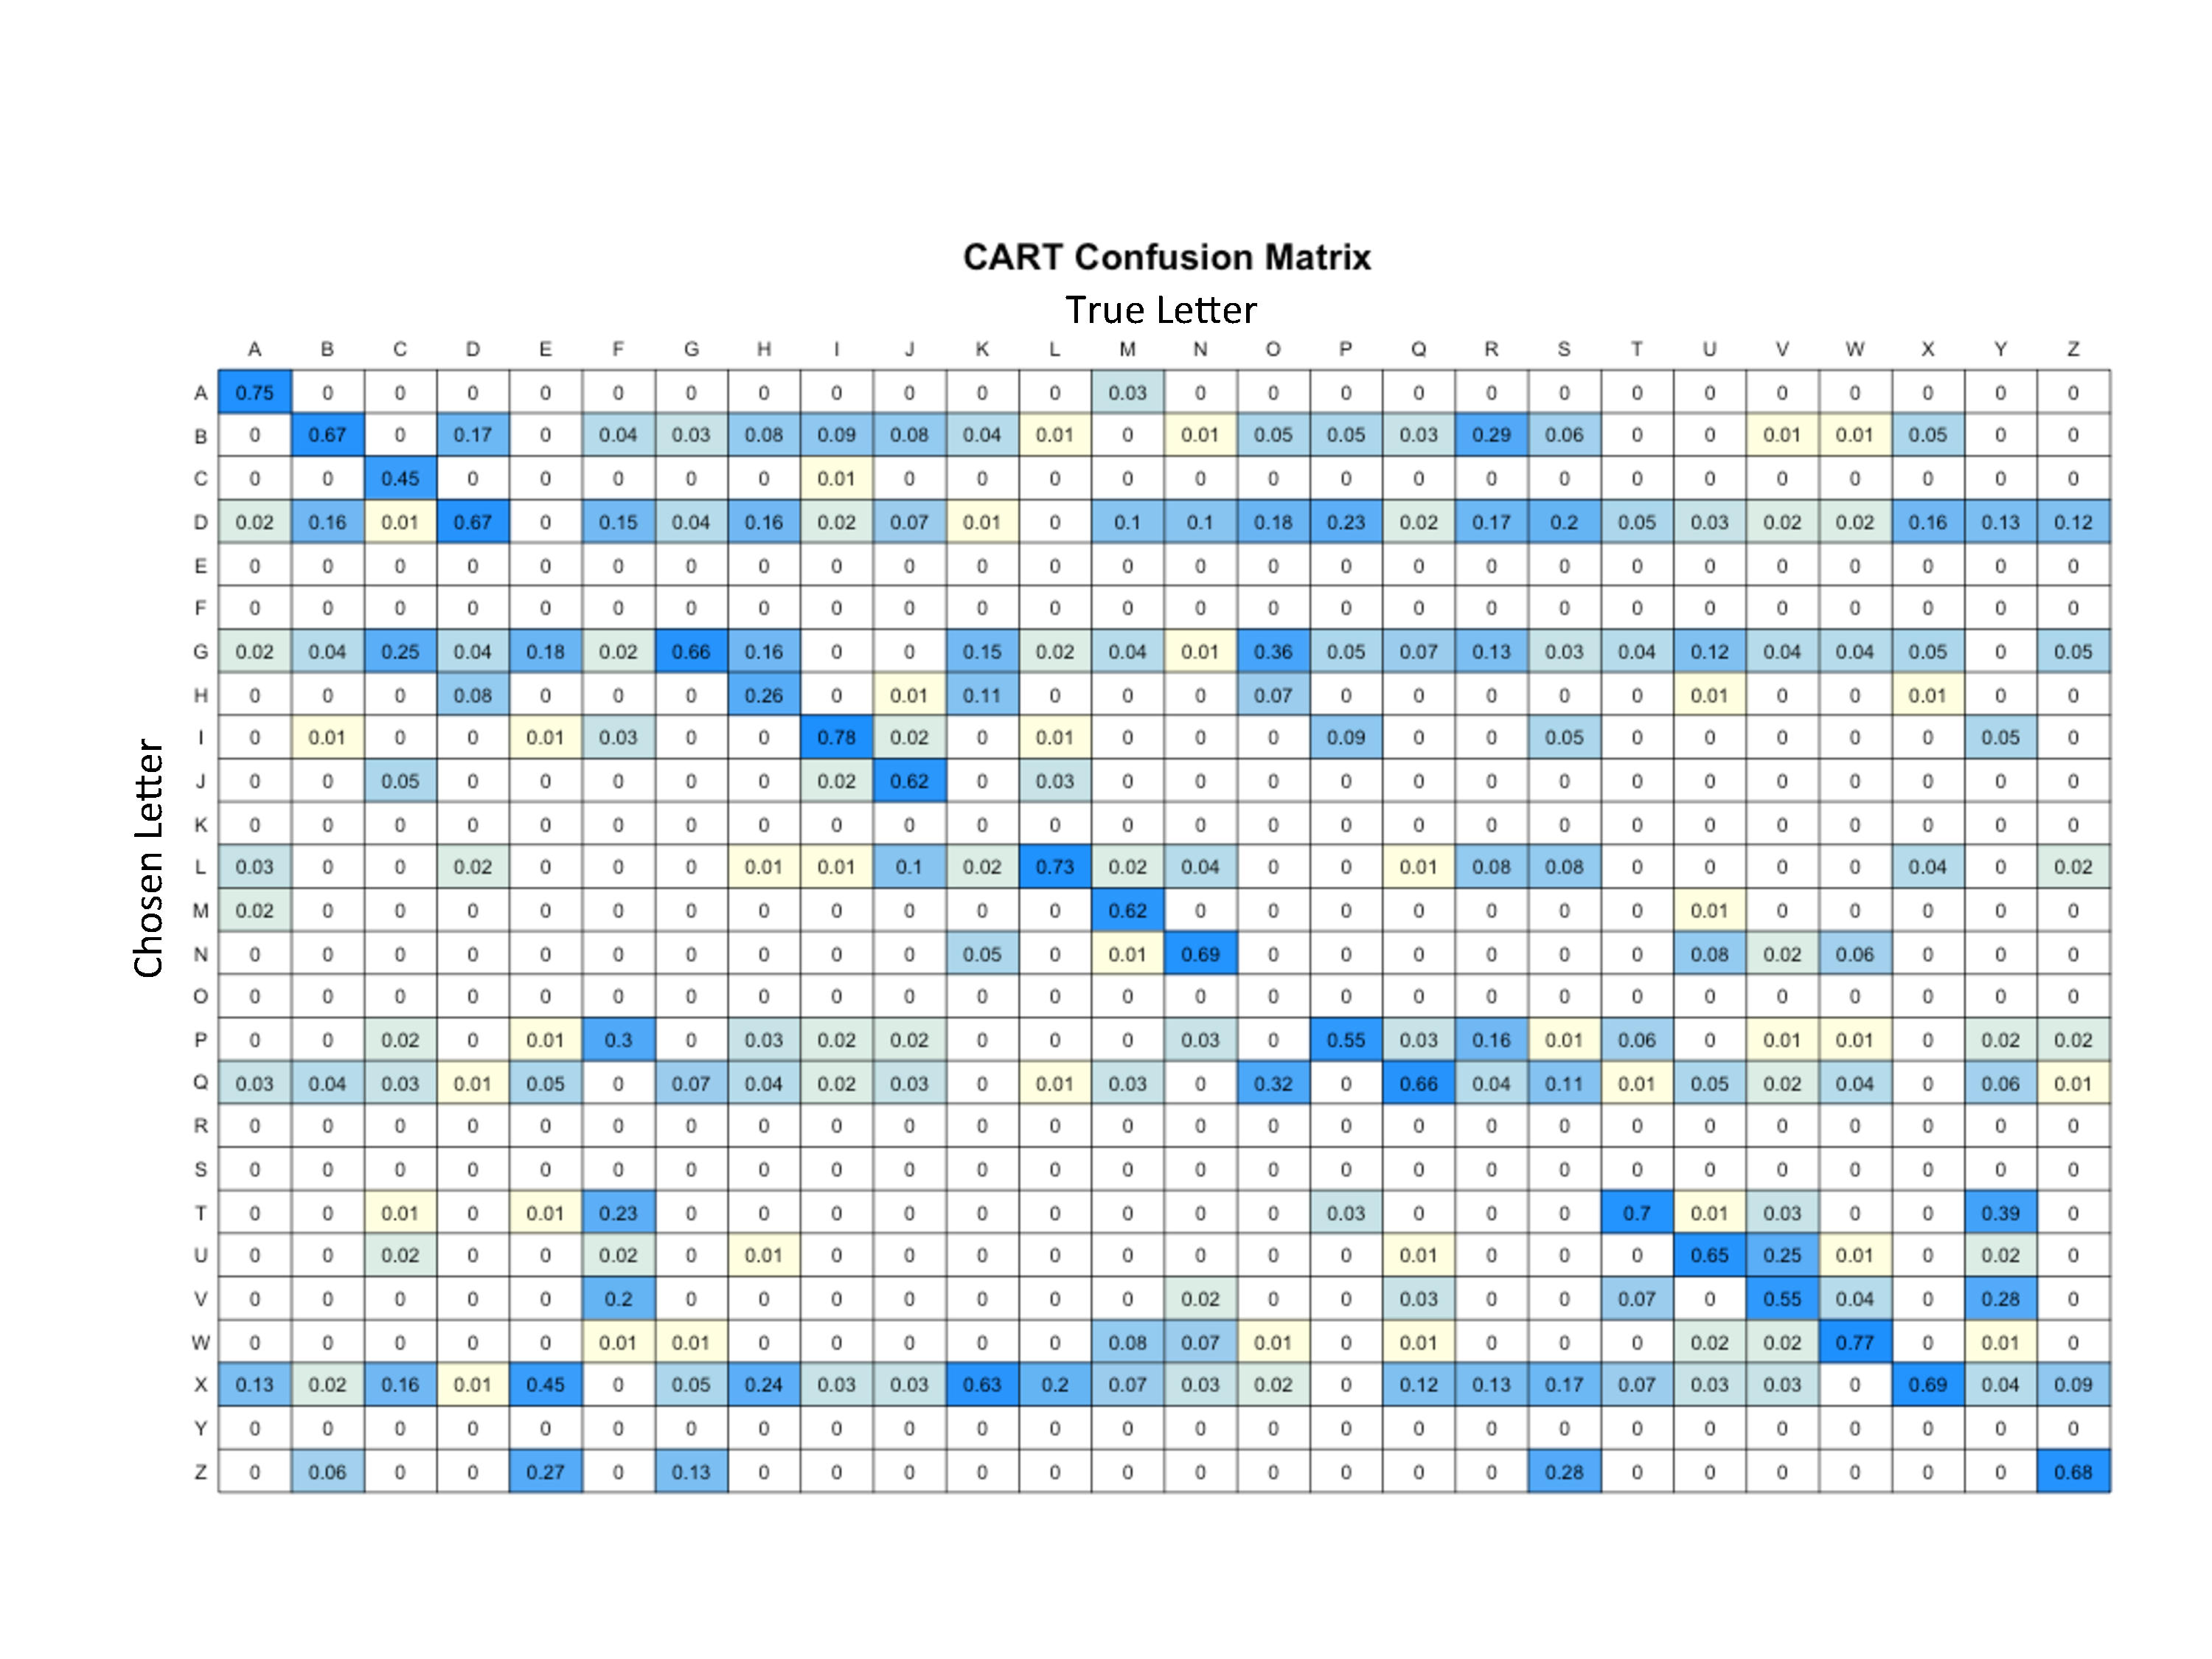
\includegraphics[width=.9 \textwidth]{cartConfuse}
\end{center}
\end{frame}

\begin{frame}
\frametitle{BAG Method Distribution of Specification}
\begin{center} 
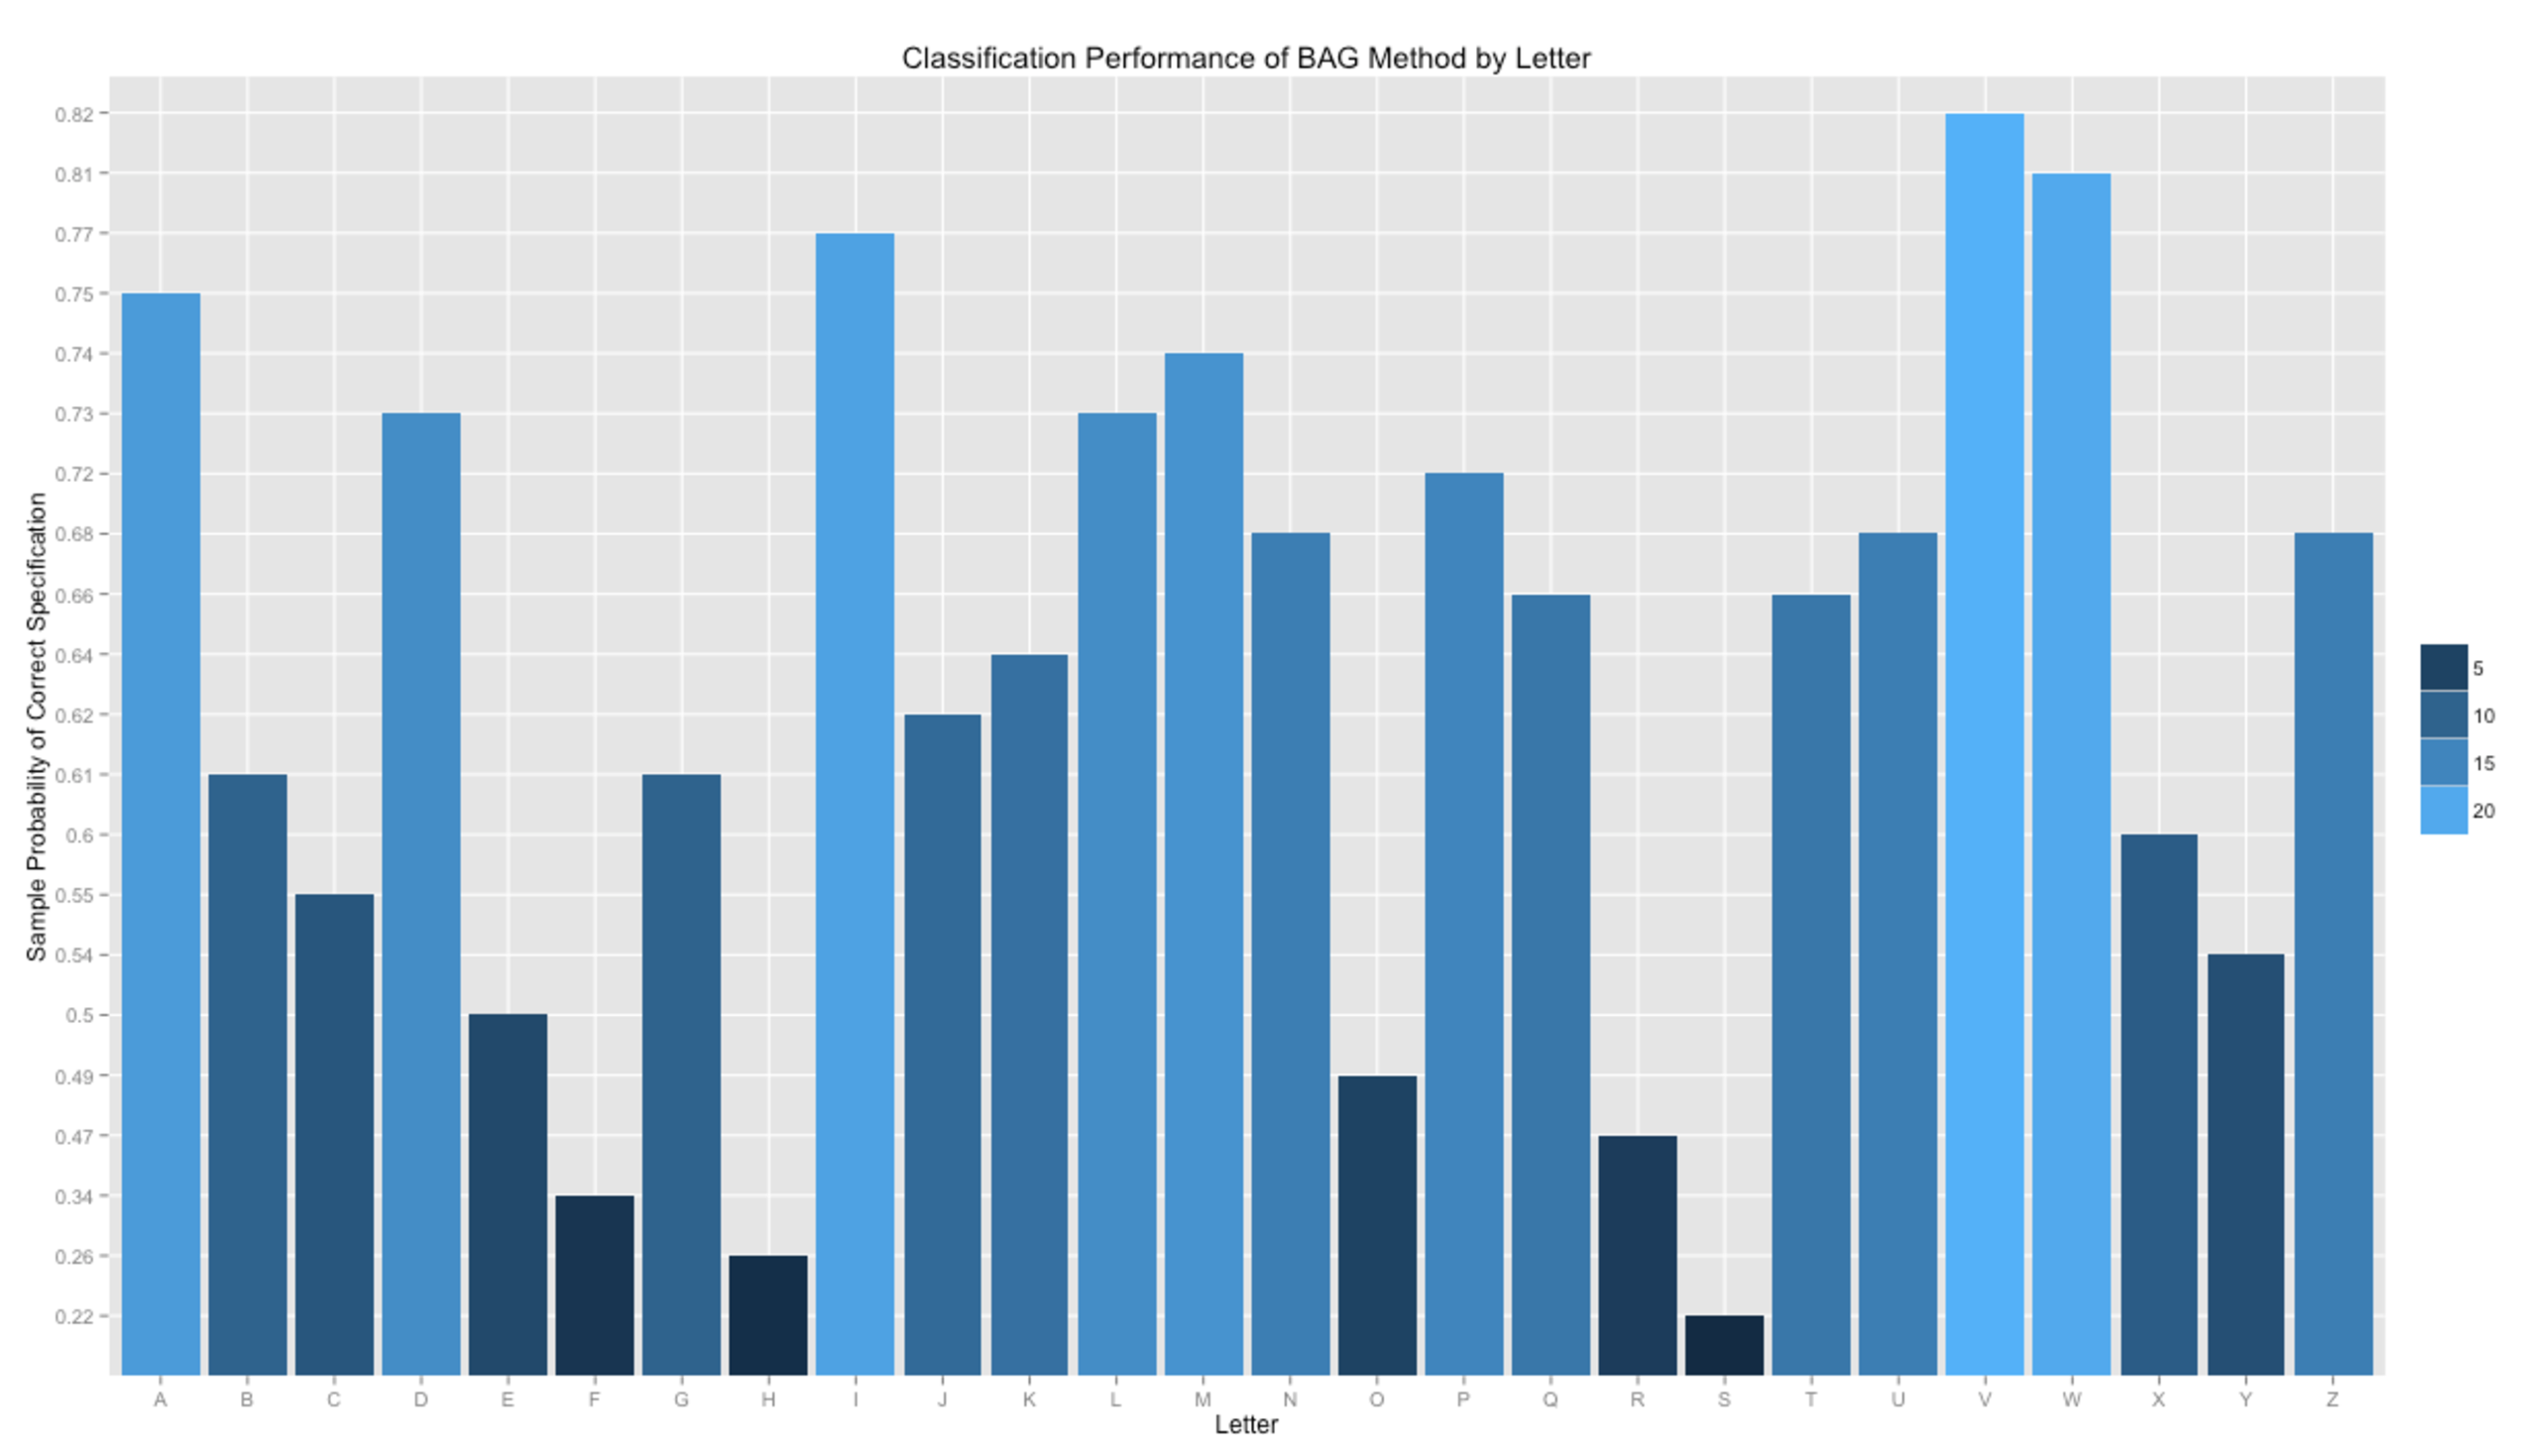
\includegraphics[width=1 \textwidth]{bagPlot}
\end{center}
\end{frame}


\begin{frame}
\frametitle{BAG Method Confusion Matrix}
\begin{center} 
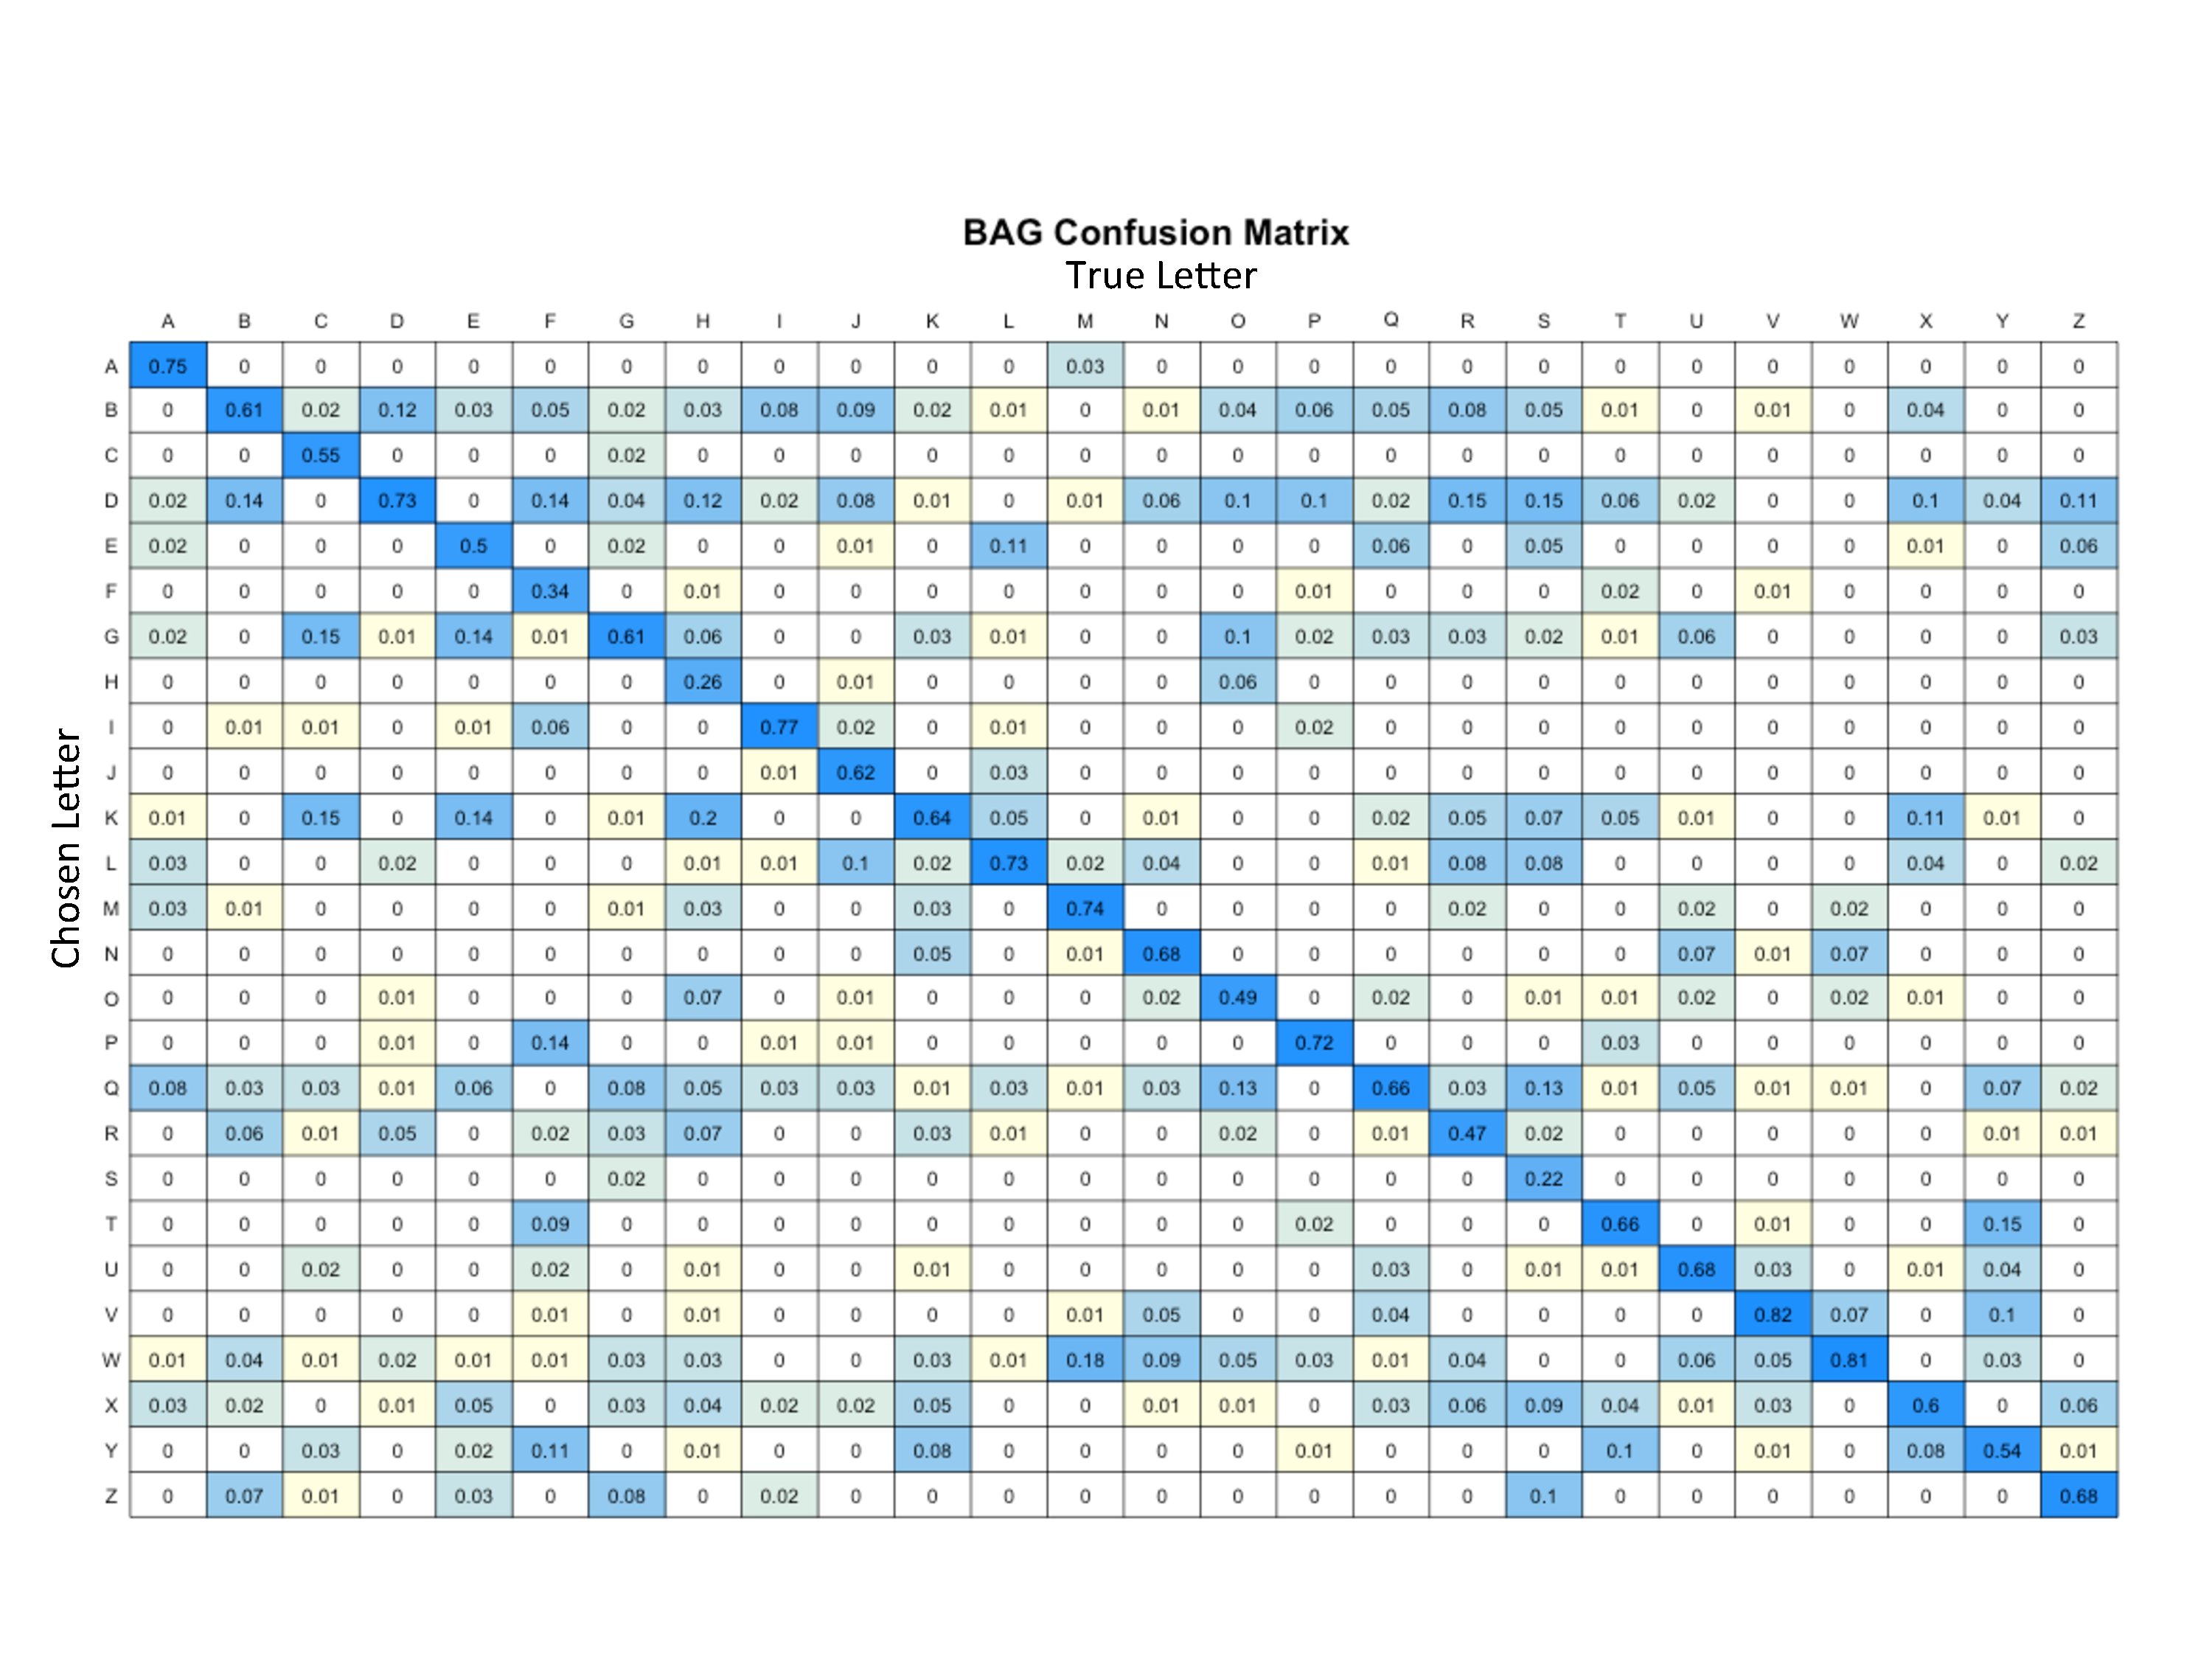
\includegraphics[width=.9 \textwidth]{bagConfuse}
\end{center}
\end{frame}


\section{Discussion}
\begin{frame}
\frametitle{Discussion}
\begin{itemize}
\item Logistic Regression Assumptions
\item Decision Tree Assumptions 
\item Scalabilty 
\end{itemize}
\end{frame}

\subsection{Logistic Regression Assumptions}
\begin{frame}
\frametitle{Usual Logistic Regression Assumptions}
\begin{itemize}
\item The true conditional probabilities are a logistic function of the independent variables
\item No important variables are omitted.
\item No extraneous variables are included.
\item The independent variables are measured without error.
\item The observations are independent.
\item The independent variables are not linear combinations of each other.
\end{itemize}

\tiny{Source: IDRE UCLA (Institute for Digital Research and Education}
\end{frame}

\subsection{Decision Tree Assumptions}
\begin{frame}
\frametitle{Decision Tree Assumptions}
CART assumptions:
\begin{enumerate}
\item Data are drawn independently from the same distribution.
\item Data is fixed and free of measurement error.
\item For classification trees the response must be discrete and the covariates are categorical, discrete, or can be discretized.
\end{enumerate}
Bagging assumptions:
\begin{enumerate}
\item The underlying classifier has small bias
\item The underlying classifier is appropriate for the data
\end{enumerate}
\end{frame}


\subsection{Scalability}
\begin{frame}
\frametitle{Scalability}
\begin{itemize}
\item Both algorithms can be applied to bigger/different data sets 
\item However, more observations and/or more categories would increase run time 
\begin{itemize}
\item LRBST already takes a long time to run ($\sim 8$ hrs) due to inefficient coding 
\item Dicision trees run quickly because there are pre-packaged functions in R. 
\item Might take more time to prune. 
\end{itemize}
\end{itemize}
\end{frame}


\subsection{Future Work}
\begin{frame}
\frametitle{Future Work}
\begin{itemize}
\item Make LRBST code more efficient by using object oriented programming aspects of R 
\item Decision trees with linear combinations of variables instead of splitting by variables one at a time 
\item Look at different letter cases, languages, symbols,...
\end{itemize}
\end{frame}




\section{Questions}
\begin{frame}
\frametitle{Questions}
\begin{center}
\begin{center} 
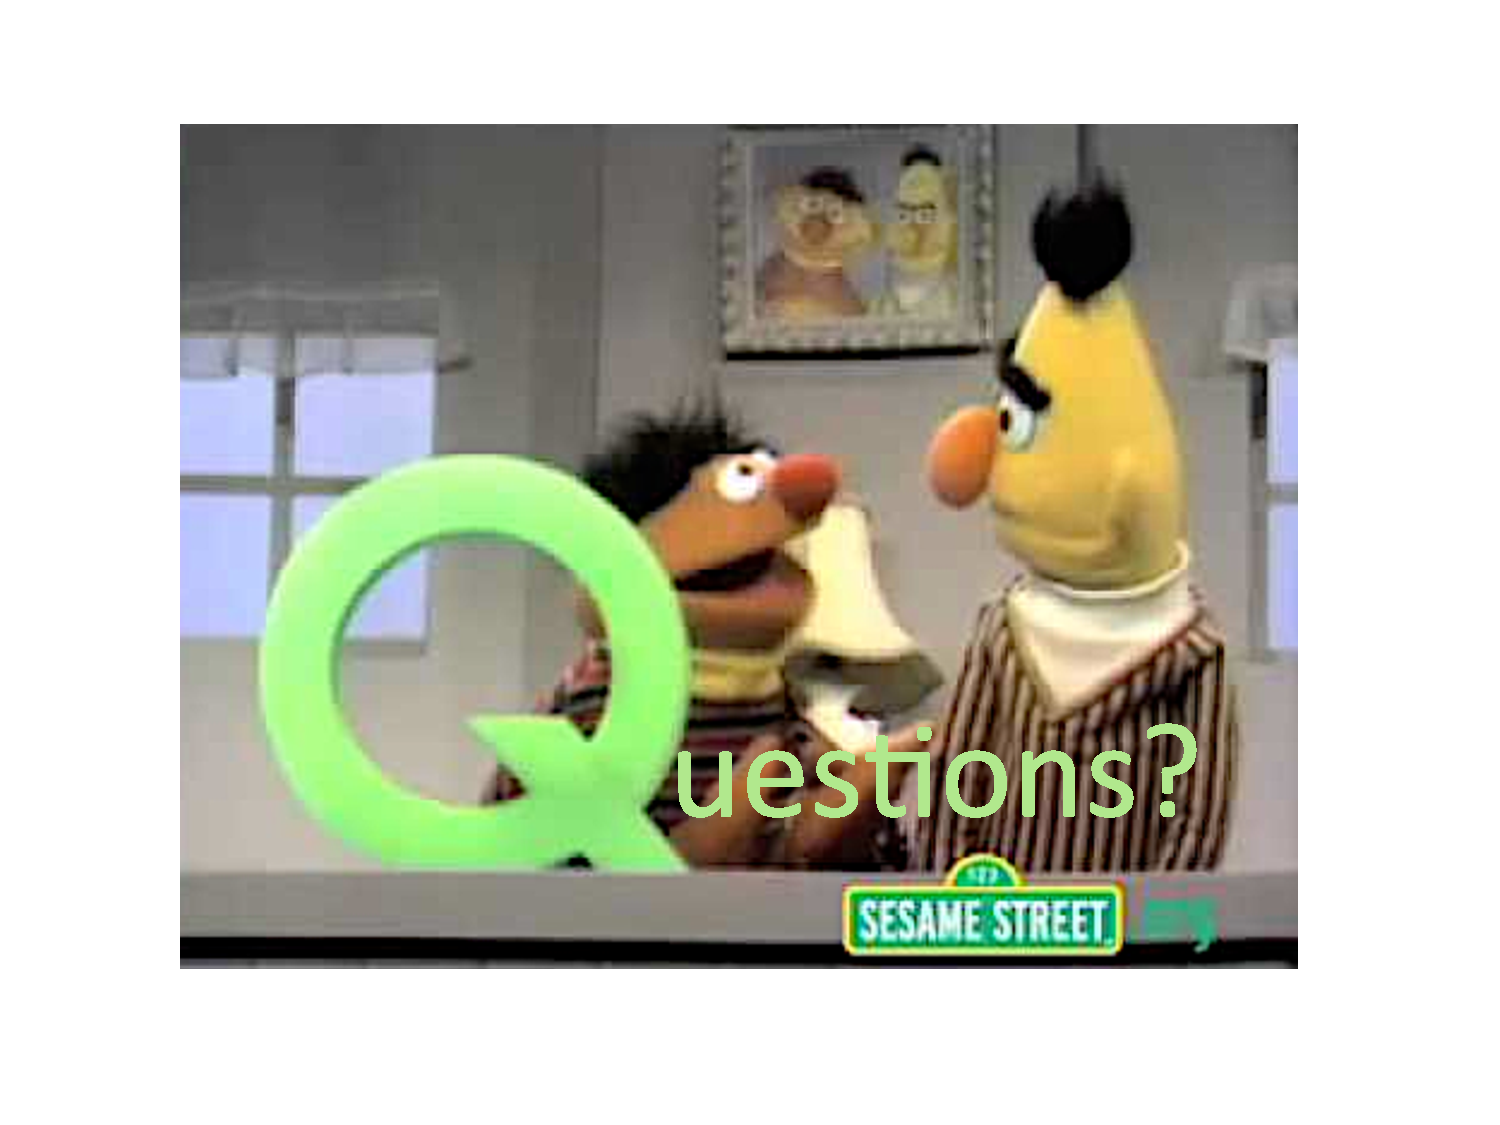
\includegraphics[width=.7 \textwidth]{quests}
\end{center}
\end{center}



\end{frame}

%\begin{center} 
%\includegraphics[width=1 \textwidth]{fieldmap}
%\end{center}
 






\end{document}
